\section{Influence of Loss Objectives on the Preservation of In-Between Instances} \label{sec:rq2}

In order to address the second research question, \textit{to what extent does augmenting the reconstruction objective of autoencoders enhance the model’s ability to capture in-between instances (IBIs)}, a systematic evaluation of different loss functions was conducted. The experimental setup builds directly on the architectural choices established in the previous section \ref{sec:rq1}. For the two-dimensional datasets, the autoencoder was configured with a network structure of 2–32–16–8–1, while for the three-dimensional datasets, a larger model with layers 3–64–32–16–2 was employed. In both cases, the Adam optimizer was used to update the weights, and scaled exponential linear units (SELU) were chosen as activation functions to ensure stable behavior throughout training.

Unlike the prior investigations into network depth and width, here the architecture was held fixed and the loss function was treated as the primary variable of interest, since the research question directly concerns the influence of the reconstruction objective. Four different losses were considered: mean squared error (MSE), cosine similarity, Kullback–Leibler divergence (KLD), and soft trustworthiness (softTW). Importantly, the evaluation focused on single losses rather than combinations. The reasoning behind this choice is that when multiple objectives are applied simultaneously, the outcome tends to be dominated by trade-offs between them, without yielding genuinely new emergent behavior. By contrast, analyzing each loss in isolation provides the clearest insight into its intrinsic properties and its ability to capture both global structure and IBIs.

Because of the nature of the different objectives, the batch size and sampling strategy were also treated as variable parameters. This was particularly relevant for soft trustworthiness, which incorporates a neighborhood size k and is highly sensitive to that local relationships are sampled. To achieve meaningful embeddings, neighborhood sampling was employed for softTW, exploiting the local nature of the objective. For the other three losses, MSE, cosine similarity, and KLD, random sampling proved more effective, producing more stable embeddings and reconstructions. The sensitivity of soft trustworthiness to the parameters n (batch size) and k (neighborhood size) also meant that its results had to be interpreted with particular care, as direct comparisons of absolute loss values across experiments were not possible.

Another important aspect of the evaluation design was the decision not to restrict the analysis to the latent space alone. While the low-dimensional embeddings provide valuable information about how clusters and IBIs are represented, the reconstructions reveal whether the model has learned to faithfully capture the geometry of the original dataset. By comparing both latent and reconstructed representations, a more comprehensive picture of each loss function’s capabilities could be obtained. In particular, the reconstructions indicate whether the loss drives the network to approximate the underlying manifolds of the datasets, and whether IBIs are positioned in accordance with their transitional roles.

% 2DBlobsS
\begin{figure}[htbp]
  \centering
  % subfigure 1
  \begin{subfigure}[b]{1.0\textwidth}
    \centering
    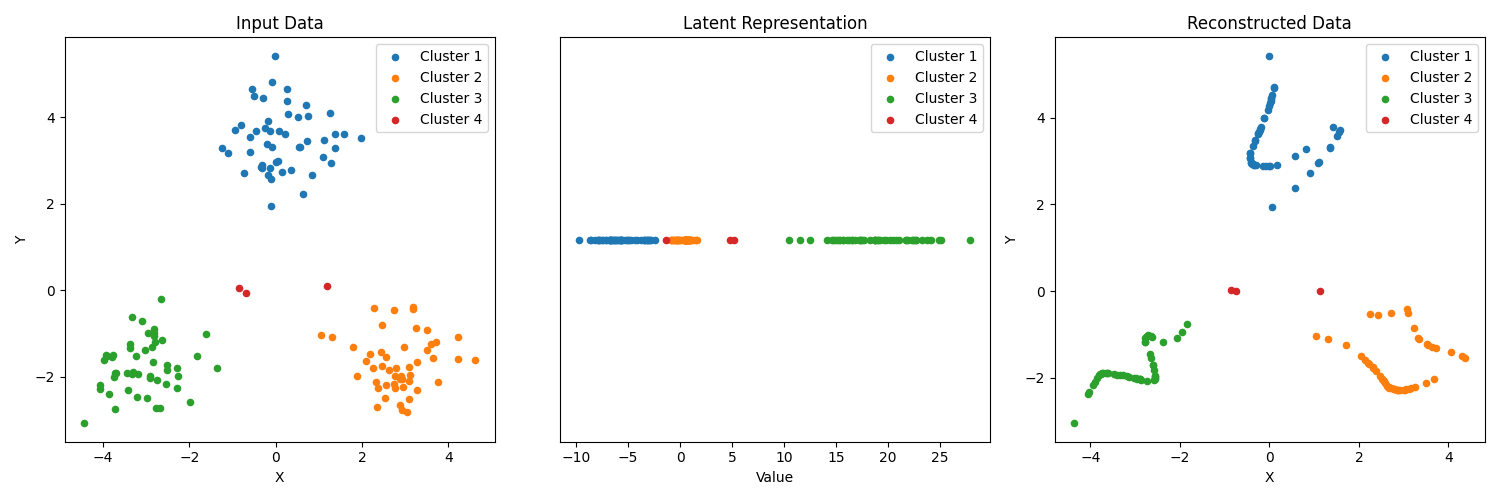
\includegraphics[width=\linewidth]{images/RQ2/mse/2DBlobsS_-1_0.0738.png}
    \caption{n=153 with 0.0738 MSE.}
    \label{fig:RQ2/mse/2DBlobsS}
  \end{subfigure}
  \hfill
  % subfigure 2
  \begin{subfigure}[b]{1.0\textwidth}
    \centering
    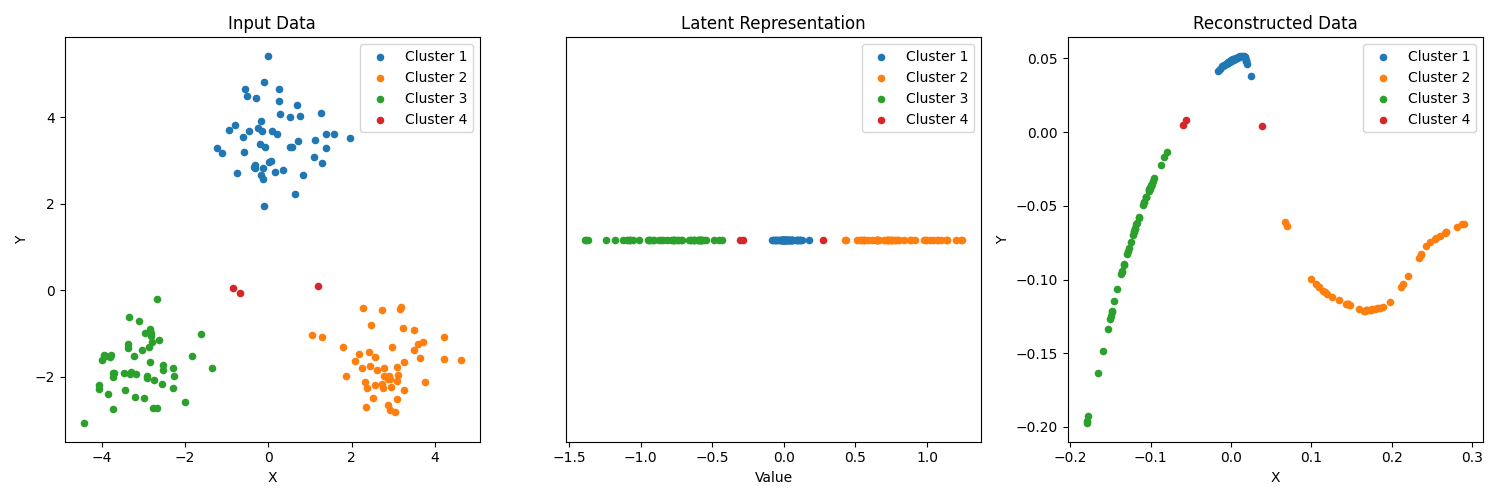
\includegraphics[width=\linewidth]{images/RQ2/csi/2DBlobsS_-1_0.0013.png}
    \caption{n=153 with 0.0641 CosSim.}
    \label{fig:RQ2/csi/2DBlobsS}
  \end{subfigure}
  \hfill
  % subfigure 3
  \begin{subfigure}[b]{1.0\textwidth}
    \centering
    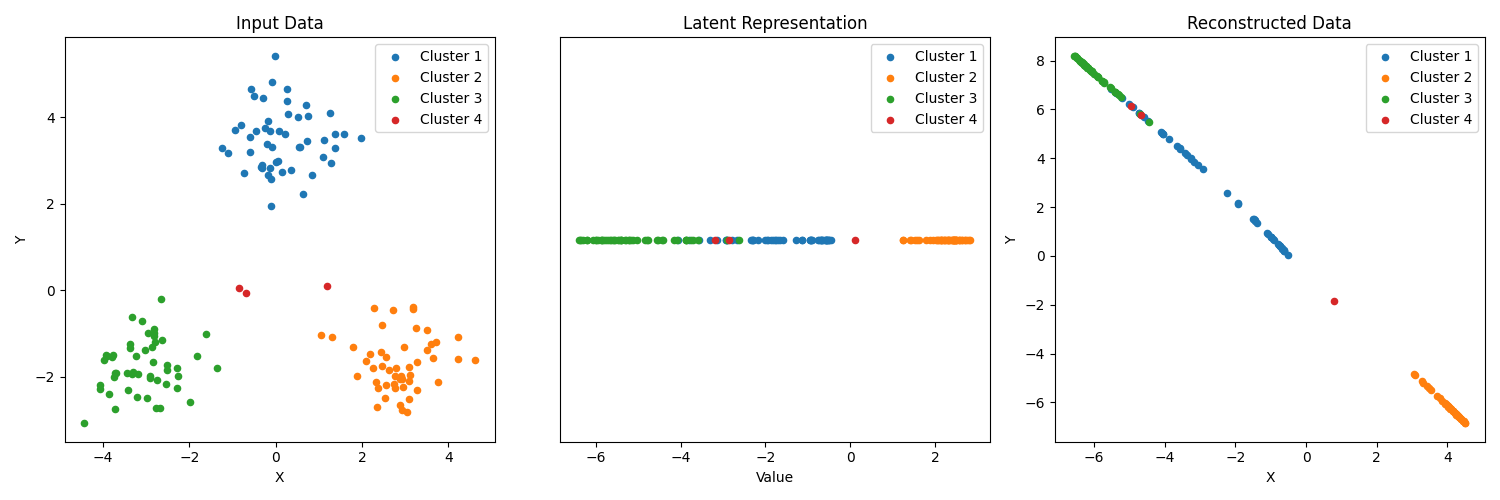
\includegraphics[width=\linewidth]{images/RQ2/kld/2DBlobsS_-1_0.0001.png}
    \caption{n=153 with 0.0001 KLD.}
    \label{fig:RQ2/kld/2DBlobsS}
  \end{subfigure}
  \hfill
  % subfigure 4
  \begin{subfigure}[b]{1.0\textwidth}
    \centering
    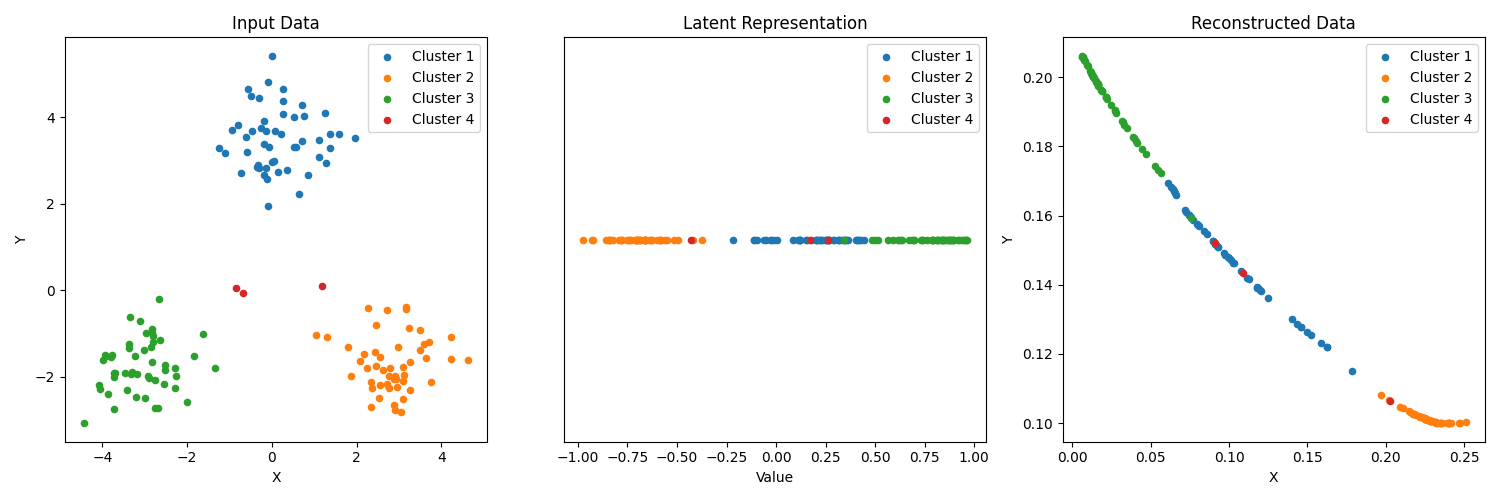
\includegraphics[width=\linewidth]{images/RQ2/tru/2DBlobsS_32n_4k_4.0776.png}
    \caption{n=32, k=4 with 4.0776 softTW.}
    \label{fig:RQ2/tru/2DBlobsS}
  \end{subfigure}

  \caption{Comparison of 2DBlobsS dataset (153 instances) experiments with different unsupervised loss functions.}
  \label{fig:RQ2/2DBlobsS}
\end{figure}

The \textbf{2DBlobsS} (Dataset \ref{fig:2DBlobsS}, Experiment \ref{fig:RQ2/2DBlobsS}) dataset represents the simplest case in the experimental setup, consisting of three well-separated Gaussian clusters with a small number of in-between instances (IBIs) positioned between them. Because of its simplicity, it provides a controlled environment for examining how different loss functions shape latent embeddings and reconstructions under identical architectural configurations. It is important to note that across all four losses, none of the models manages to reproduce the dataset perfectly. Instead, the reconstructions consistently lie on manifolds of varying complexity, which cannot be attributed to architectural differences since the configurations were held constant.

In the latent space, both mean squared error (MSE) and cosine similarity produce near-perfect embeddings. The clusters are clearly separated, and the IBIs are positioned correctly in transitional regions, which reflects the intended structural role of these instances. The Kullback–Leibler divergence also performs reasonably well in the latent space, but here some shortcomings become visible: the blue and green clusters begin to overlap, and the IBI situated between them is no longer represented with the same clarity as under MSE or cosine similarity. The weakest embedding emerges with the soft trustworthiness loss, which produces more overlapping between clusters and a less distinct placement of IBIs. Nevertheless, even in this case the two-dimensional embeddings remain sufficiently informative, and it would not be accurate to describe any of the losses as performing badly on this relatively simple dataset.

The more pronounced differences appear in the reconstructions. MSE produces the most complex reconstruction, where the data is distributed across several manifold-like curves to approximate the original arrangement of clusters. This reconstruction maintains strong fidelity to the dataset’s underlying structure, and the IBIs are placed with particular accuracy, bridging the appropriate clusters. Cosine similarity results in a less complex reconstruction: the points lie on a single manifold that is curved, reflecting the global continuity it enforces but at the cost of reducing local geometric richness. The reconstructions generated by KLD and soft trustworthiness collapse further, lying essentially on one-dimensional manifolds. These are the least complex structures that can emerge in this setting, yet for such a simple dataset they are still able to capture the main separations between clusters and maintain a usable representation of IBIs.

Overall, the analysis of 2DBlobsS shows that while all four losses are adequate for producing workable embeddings in simple scenarios, they diverge significantly in how they reconstruct the data. MSE emerges as the most faithful, capable of mimicking the dataset’s original geometry through complex manifolds while also positioning IBIs with high precision. Cosine similarity offers a simpler but still reasonable reconstruction, whereas KLD and soft trustworthiness reduce the geometry to overly simplified one-dimensional forms. For this dataset, these reductions are not catastrophic, but they reveal the limitations of the latter losses in capturing more global geometries. The findings suggest that, at least for simple data, all four losses are sufficient in low-dimensional embeddings, but MSE stands out in balancing embedding quality with structurally faithful reconstructions.

% 2DBlobsM
\begin{figure}[htbp]
  \centering
  % subfigure 1
  \begin{subfigure}[b]{1.0\textwidth}
    \centering
    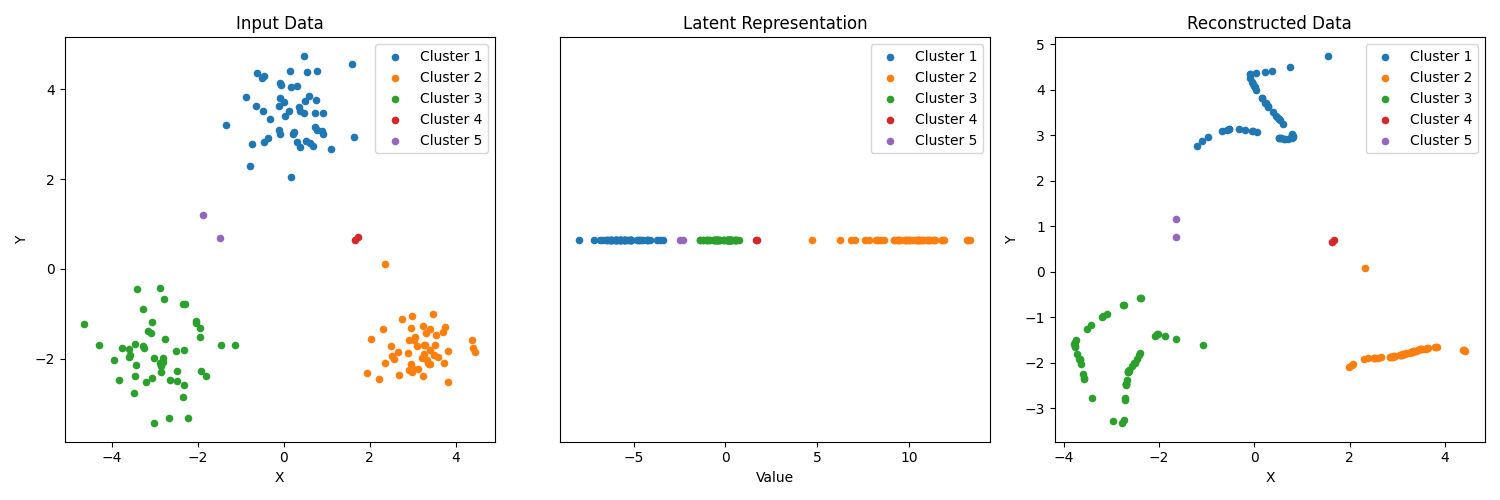
\includegraphics[width=\linewidth]{images/RQ2/mse/2DBlobsM_-1_0.0646.png}
    \caption{n=154 with 0.0646 MSE.}
    \label{fig:RQ2/mse/2DBlobsM}
  \end{subfigure}
  \hfill
  % subfigure 2
  \begin{subfigure}[b]{1.0\textwidth}
    \centering
    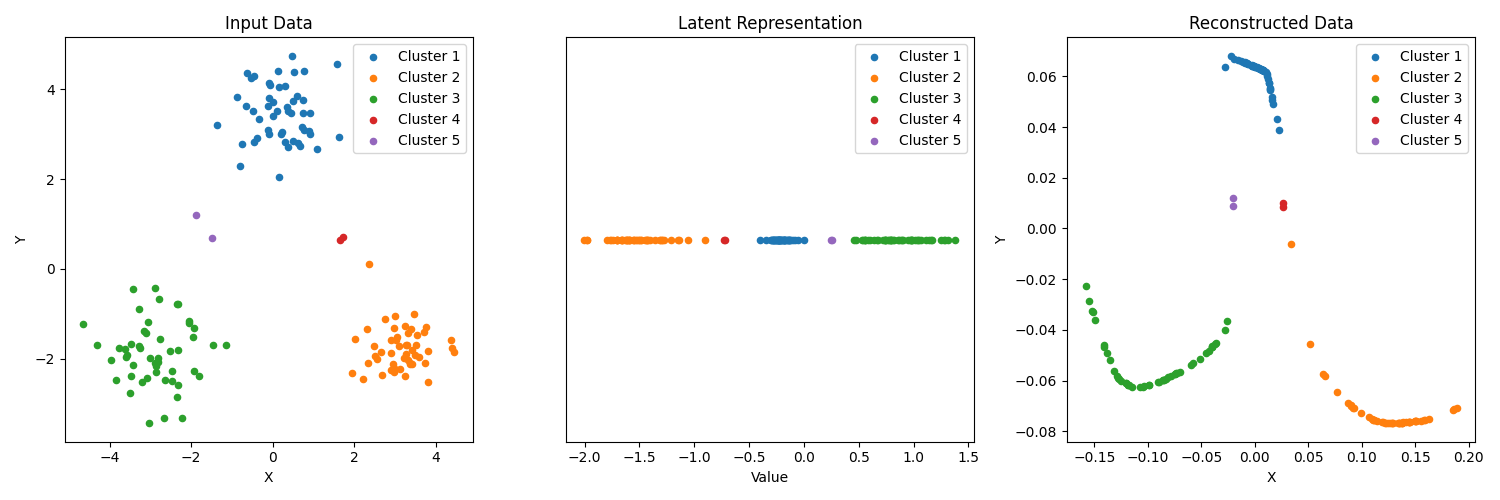
\includegraphics[width=\linewidth]{images/RQ2/csi/2DBlobsM_-1_0.0014.png}
    \caption{n=154 with 0.0014 CosSim.}
    \label{fig:RQ2/csi/2DBlobsM}
  \end{subfigure}
  \hfill
  % subfigure 3
  \begin{subfigure}[b]{1.0\textwidth}
    \centering
    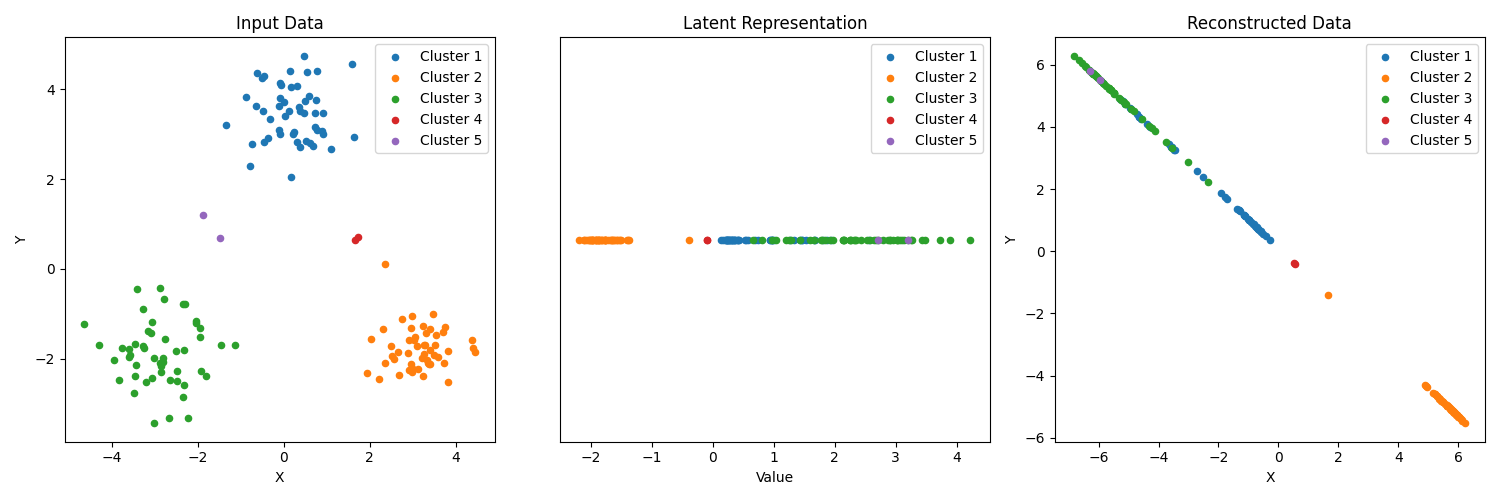
\includegraphics[width=\linewidth]{images/RQ2/kld/2DBlobsM_-1_0.0001.png}
    \caption{n=154 with 0.0001 KLD.}
    \label{fig:RQ2/kld/2DBlobsM}
  \end{subfigure}
  \hfill
  % subfigure 4
  \begin{subfigure}[b]{1.0\textwidth}
    \centering
    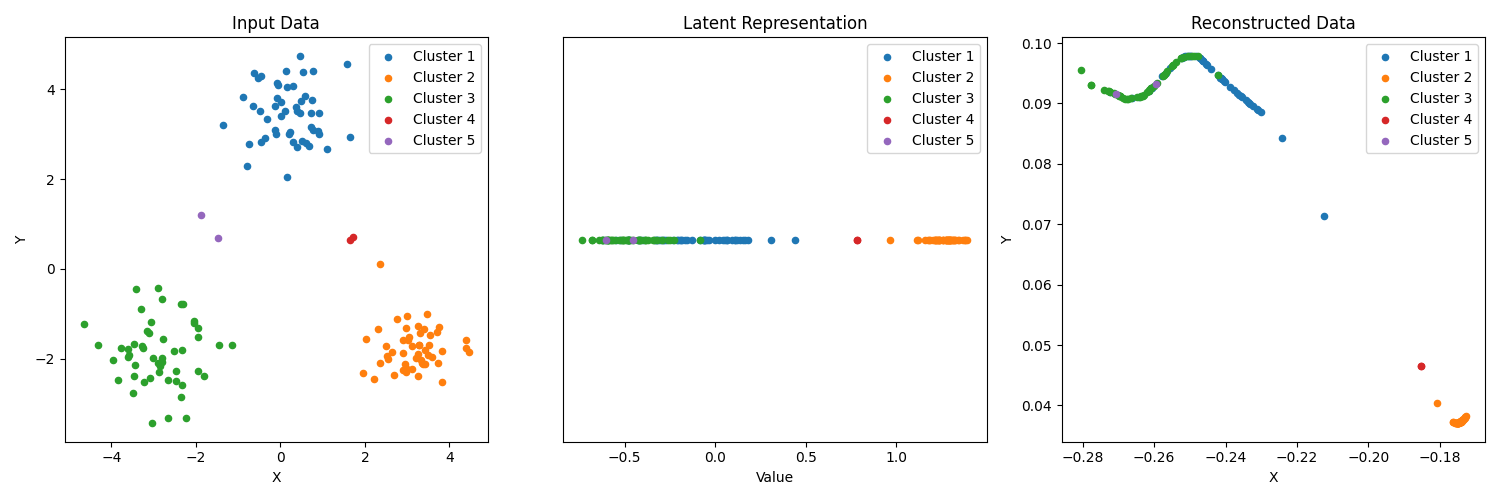
\includegraphics[width=\linewidth]{images/RQ2/tru/2DBlobsM_32n_4k_4.0777.png}
    \caption{n=32, k=4 with 4.0777 softTW.}
    \label{fig:RQ2/tru/2DBlobsM}
  \end{subfigure}

  \caption{Comparison of 2DBlobsM dataset (154 instances) experiments with different unsupervised loss functions.}
  \label{fig:RQ2/2DBlobsM}
\end{figure}

The \textbf{2DBlobsM} (Dataset \ref{fig:2DBlobsM}, Experiment \ref{fig:RQ2/2DBlobsM}) dataset was originally designed as an extension of 2DBlobsS to emphasize IBIs that emerge between pairs of clusters rather than from a single distribution located centrally. While 2DBlobsS contains transitional points that could plausibly be understood as belonging to one underlying distribution bridging all clusters, 2DBlobsM introduces two distinct sets of IBIs, each situated between a different pair of clusters. In theory, this makes it a more challenging case for autoencoders, as the embeddings must capture not just one transitional structure but two, each connecting different groups. In practice, however, the dataset’s overall geometry remains highly similar to 2DBlobsS, and as a result, the outcomes across the four losses resemble those observed in the simpler case, with only minor but instructive differences.

As in the previous dataset, MSE and cosine similarity both yield strong latent embeddings. The clusters are well separated, and the IBIs occupy transitional positions, though the embeddings do not provide additional clarity beyond what was already observed in 2DBlobsS. KLD again produces a weaker representation, with partial overlap of clusters that obscures the intended transitional structure. The soft trustworthiness loss, however, diverges from the earlier pattern. In this case, it produces a more complex reconstruction, which initially suggests an improved ability to capture the dataset’s underlying structure. Yet this increased complexity in the reconstruction does not translate into a more meaningful latent representation. While the red IBIs are positioned more convincingly between the yellow and blue clusters, fulfilling their intended role as transitional instances, the purple IBIs are handled poorly. Instead of appearing between the green and blue clusters, as designed, they are placed within the green cluster itself, thereby losing their transitional character and obscuring their bridging function.

These results highlight the nuanced but significant ways in which loss functions can interact with subtle changes in dataset design. While all four losses behaved similarly to their performance on 2DBlobsS, the soft trustworthiness loss illustrates a limitation in its consistency: it may succeed in positioning one set of IBIs appropriately while failing to preserve another, even when both are present in the same dataset. This suggests that although the local-neighborhood emphasis of soft trustworthiness can sometimes improve the fidelity of individual transitional structures, it does not guarantee a globally coherent treatment of all IBIs within a dataset. By contrast, MSE and cosine similarity continue to provide robust, if unspectacular, embeddings that preserve both clusters and transitional points in a manner that is reliable across similar datasets. The findings for 2DBlobsM therefore reinforce the conclusions drawn from 2DBlobsS, while also emphasizing the potential inconsistency of structure-preserving losses when applied to datasets with multiple sets of IBIs.

% 2DMoons
\begin{figure}[htbp]
  \centering
  % subfigure 1
  \begin{subfigure}[b]{1.0\textwidth}
    \centering
    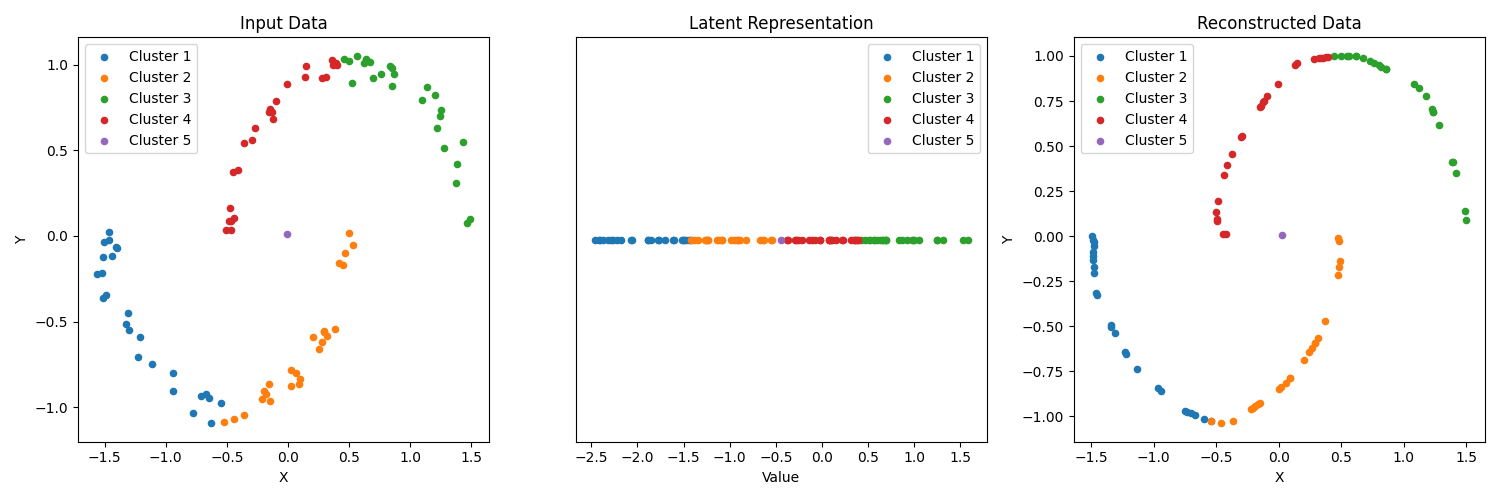
\includegraphics[width=\linewidth]{images/RQ2/mse/2DMoons_-1_0.0014.png}
    \caption{n=101 with 0.0014 MSE.}
    \label{fig:RQ2/mse/2DMoons}
  \end{subfigure}
  \hfill
  % subfigure 2
  \begin{subfigure}[b]{1.0\textwidth}
    \centering
    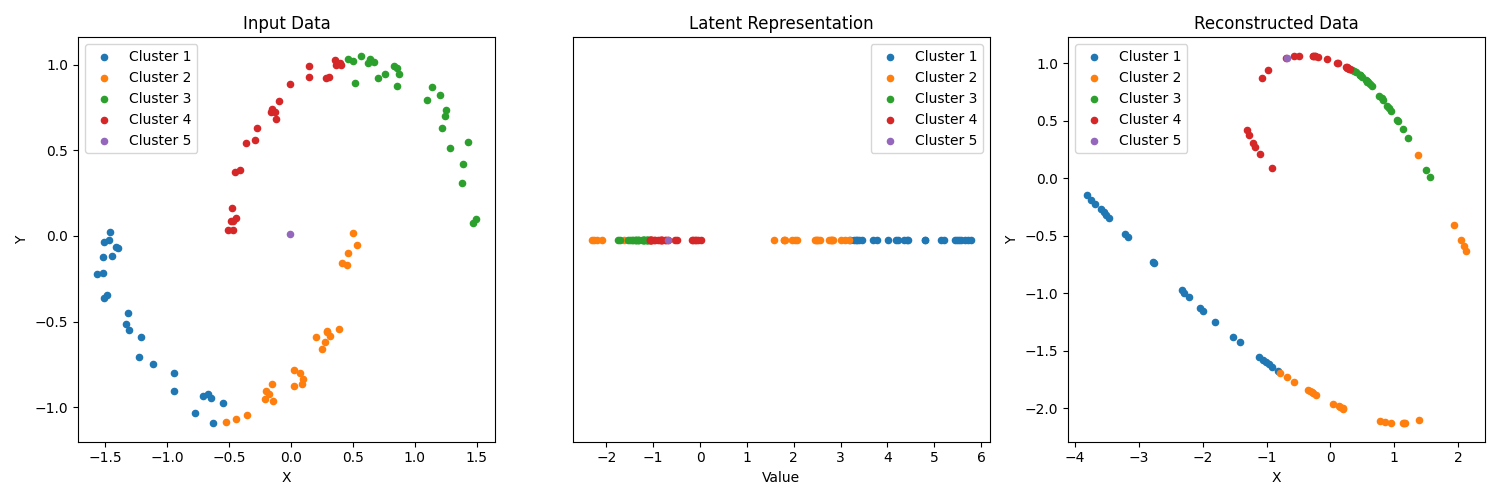
\includegraphics[width=\linewidth]{images/RQ2/csi/2DMoons_2_0.0008.png}
    \caption{n=101 with 0.0008 CosSim.}
    \label{fig:RQ2/csi/2DMoons}
  \end{subfigure}
  \hfill
  % subfigure 3
  \begin{subfigure}[b]{1.0\textwidth}
    \centering
    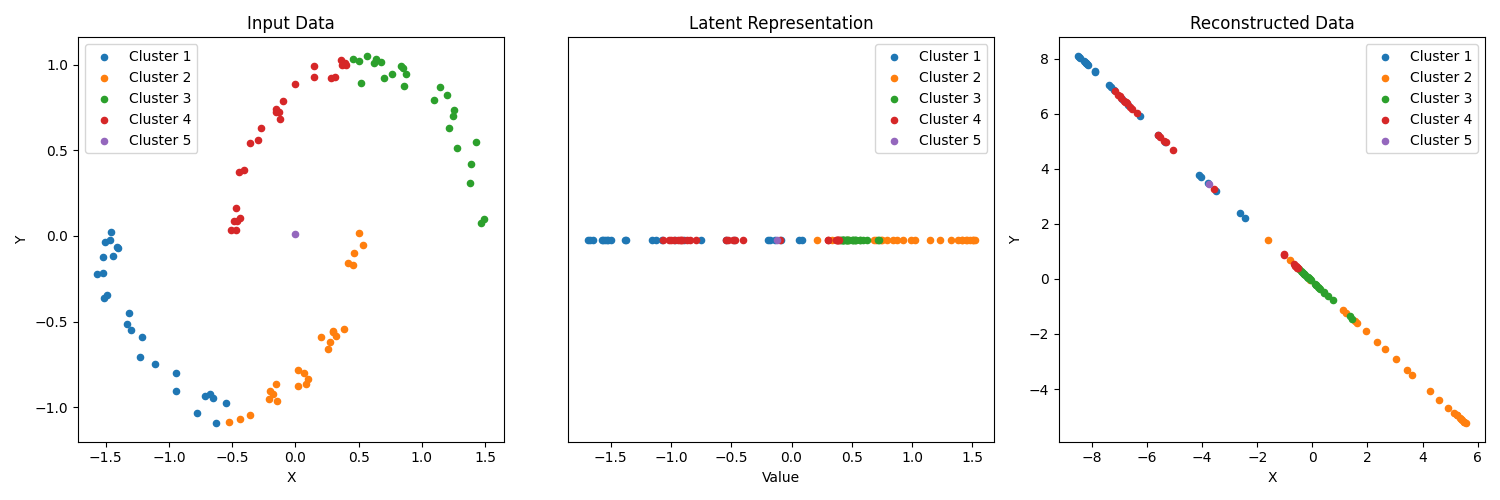
\includegraphics[width=\linewidth]{images/RQ2/kld/2DMoons_-1_0.0002.png}
    \caption{n=101 with 0.0002 KLD.}
    \label{fig:RQ2/kld/2DMoons}
  \end{subfigure}
  \hfill
  % subfigure 4
  \begin{subfigure}[b]{1.0\textwidth}
    \centering
    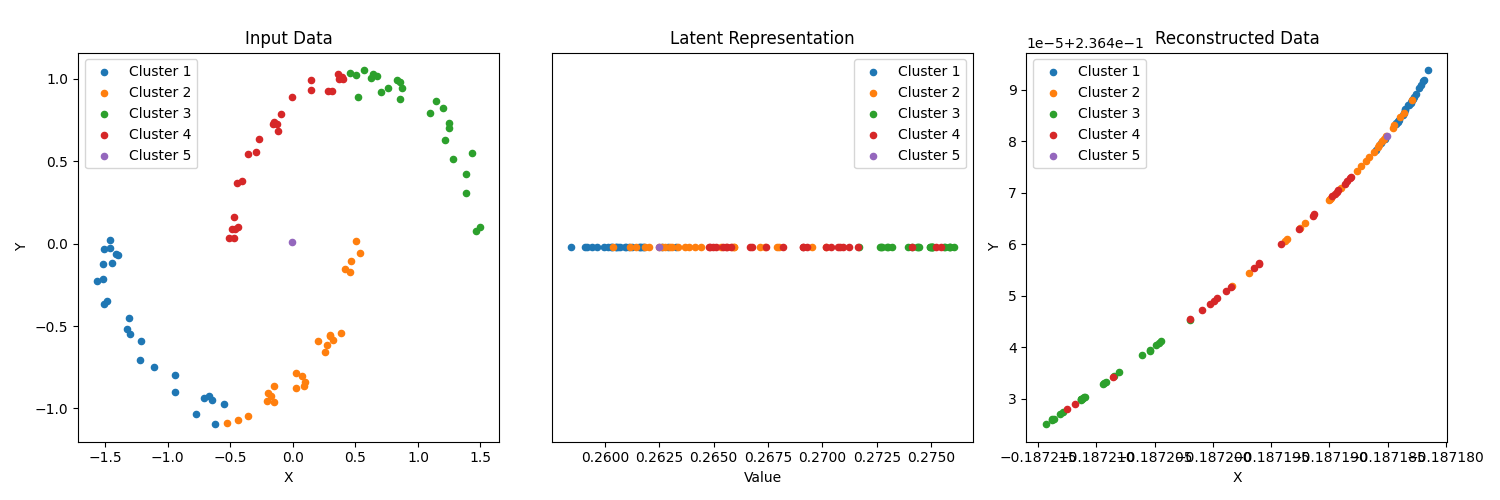
\includegraphics[width=\linewidth]{images/RQ2/tru/2DMoons_16n_8k_0.5255.png}
    \caption{n=16, k=8 with 0.5255 softTW.}
    \label{fig:RQ2/tru/2DMoons}
  \end{subfigure}

  \caption{Comparison of 2DMoons dataset (101 instances) experiments with different unsupervised loss functions.}
  \label{fig:RQ2/2DMoons}
\end{figure}

The \textbf{2DMoons} (Dataset \ref{fig:2DMoons}, Experiment \ref{fig:RQ2/2DMoons}) dataset introduces a different type of complexity compared to the blob-based datasets analyzed previously. Instead of compact Gaussian clusters, the data here consists of two concave clusters arranged in the familiar crescent or “moon” shapes, with one IBI positioned between them. This non-linear geometry places greater demands on the reconstruction process, since an effective model must capture not only cluster separation but also the curved structure of the manifolds themselves.

In terms of reconstruction, the mean squared error once again performs the strongest. The overall crescent-shaped structure of both moons is captured with high fidelity, demonstrating that the model has learned the essential global geometry of the dataset. The one notable limitation lies in the width of the reconstructed clusters, which appear overly narrow compared to the original data. This is not necessarily a shortcoming of the loss function itself but rather a structural limitation of the autoencoder, in which the dimensional compression imposed by the bottleneck layer naturally discards some finer-grained information. In contrast, the reconstructions produced by the other three losses fail to capture the moon-like structure convincingly. Cosine similarity introduces distortions that break the smooth continuity of the arcs, while KLD and soft trustworthiness both collapse the dataset onto a nearly one-dimensional manifold. This simplification eliminates the essential curvature of the moons and undermines the interpretability of the reconstructions.

The latent embeddings show a similar hierarchy of performance. Under MSE, the two moons are represented almost perfectly, with clear continuity of the arcs and the IBI correctly positioned in the transitional zone between them. The only improvement that might be suggested would be a slightly clearer separation of the IBI from the clusters themselves, which would make its bridging role more explicit. Cosine similarity provides this additional separation in the embedding, but at a cost: the IBI is misplaced, appearing within the red section of the upper moon rather than in the intended transitional space. Additionally, some of the yellow points that should form part of the lower arc are embedded behind the green section, disrupting the internal consistency of the representation. The KLD embedding displays another type of structural failure, as the order of the moon segments becomes scrambled: after the blue section, the red points appear instead of the yellow, disrupting the natural continuity of the arcs. This effect may be connected to the choice of batch size, which in this case included the full dataset. Interestingly, under this configuration KLD performed relatively better than in earlier experiments, though still far from optimal. Finally, soft trustworthiness embeds the sequence of moon segments in the correct order, which is an improvement over KLD, but fails to establish clear separation between the moons themselves or between the different colored sections of each arc. As a result, the IBI is placed poorly, appearing within the yellow section of the bottom moon rather than between the two structures.

Altogether, the analysis of 2DMoons underscores the strengths of MSE in handling both global geometry and the placement of IBIs, albeit with the expected limitations of an autoencoder bottleneck that constrains cluster width. Cosine similarity demonstrates partial advantages in separating the IBI but introduces structural inconsistencies, while KLD and soft trustworthiness fail to preserve the overall moon geometry, reducing the embeddings to simplified or scrambled forms. This dataset thus highlights more sharply than the blob datasets the risks of relying on losses that collapse structure, and it reinforces the conclusion that MSE remains the most reliable choice for preserving non-linear cluster geometries and transitional instances.

% 2DSwissRoll
\begin{figure}[htbp]
  \centering
  % subfigure 1
  \begin{subfigure}[b]{1.0\textwidth}
    \centering
    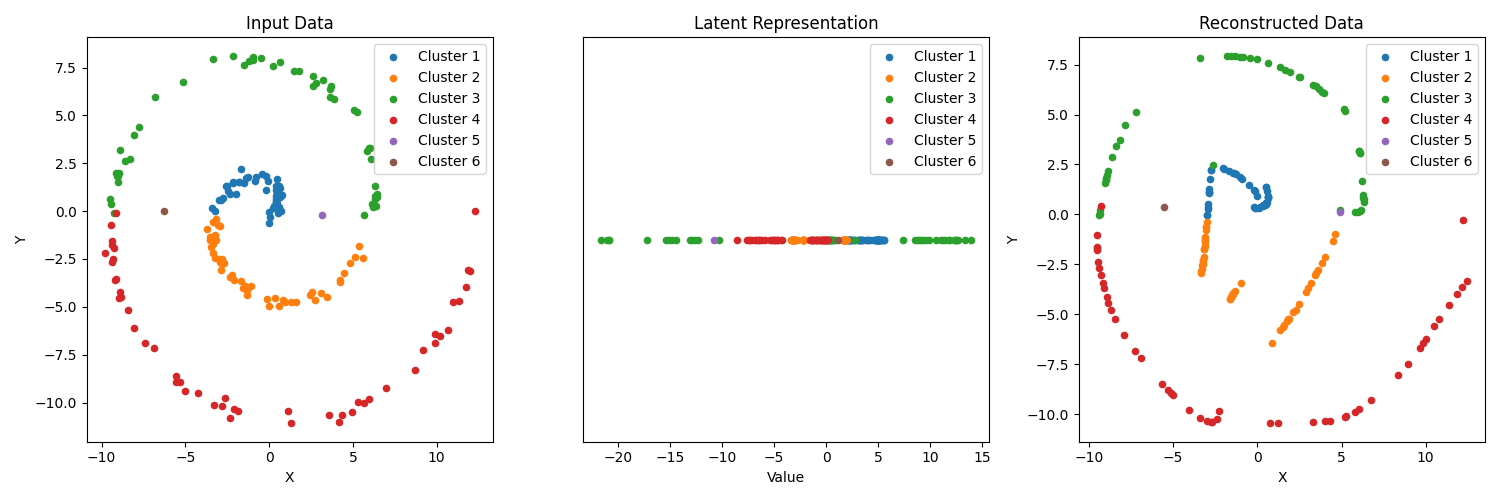
\includegraphics[width=\linewidth]{images/RQ2/mse/2DSwissRoll_-1_0.2319.png}
    \caption{n=202 with 0.2319 MSE.}
    \label{fig:RQ2/mse/2DSwissRoll}
  \end{subfigure}
  \hfill
  % subfigure 2
  \begin{subfigure}[b]{1.0\textwidth}
    \centering
    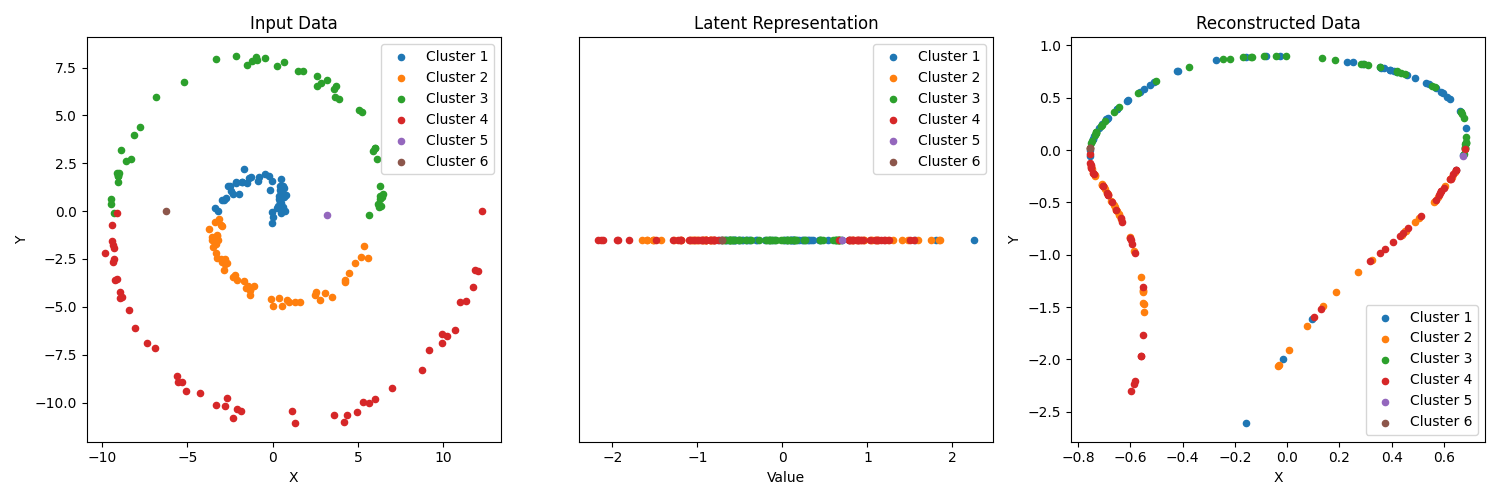
\includegraphics[width=\linewidth]{images/RQ2/csi/2DSwissRoll_2_0.0008.png}
    \caption{n=202 with 0.0008 CosSim.}
    \label{fig:RQ2/csi/2DSwissRoll}
  \end{subfigure}
  \hfill
  % subfigure 3
  \begin{subfigure}[b]{1.0\textwidth}
    \centering
    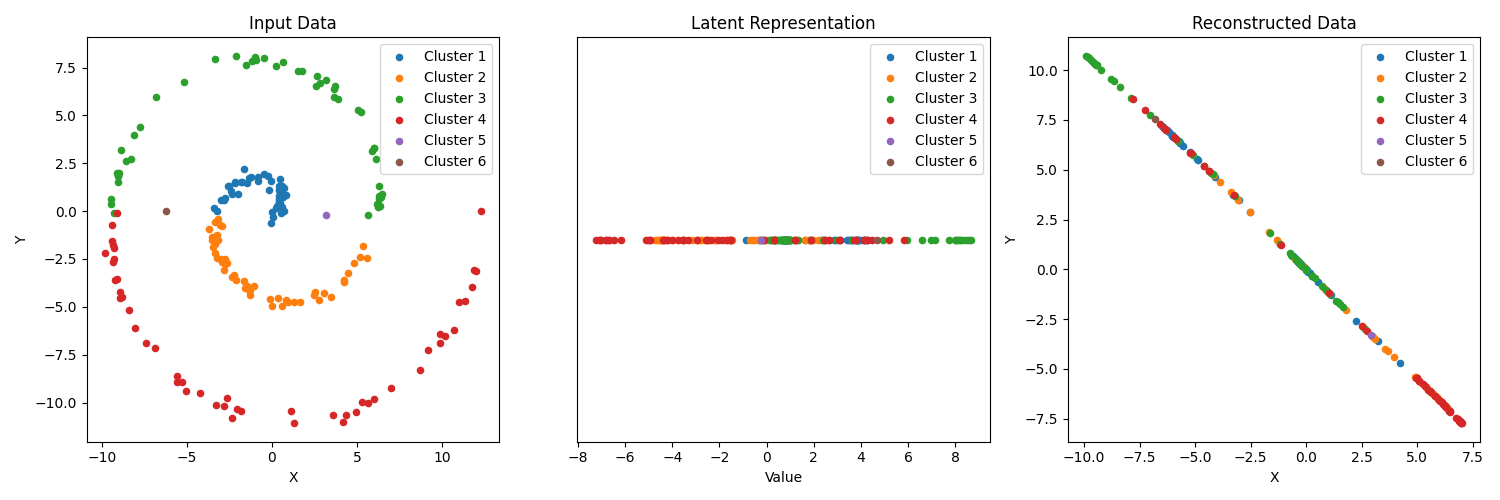
\includegraphics[width=\linewidth]{images/RQ2/kld/2DSwissRoll_-1_0.0002.png}
    \caption{n=202 with 0.0002 KLD.}
    \label{fig:RQ2/kld/2DSwissRoll}
  \end{subfigure}
  \hfill
  % subfigure 4
  \begin{subfigure}[b]{1.0\textwidth}
    \centering
    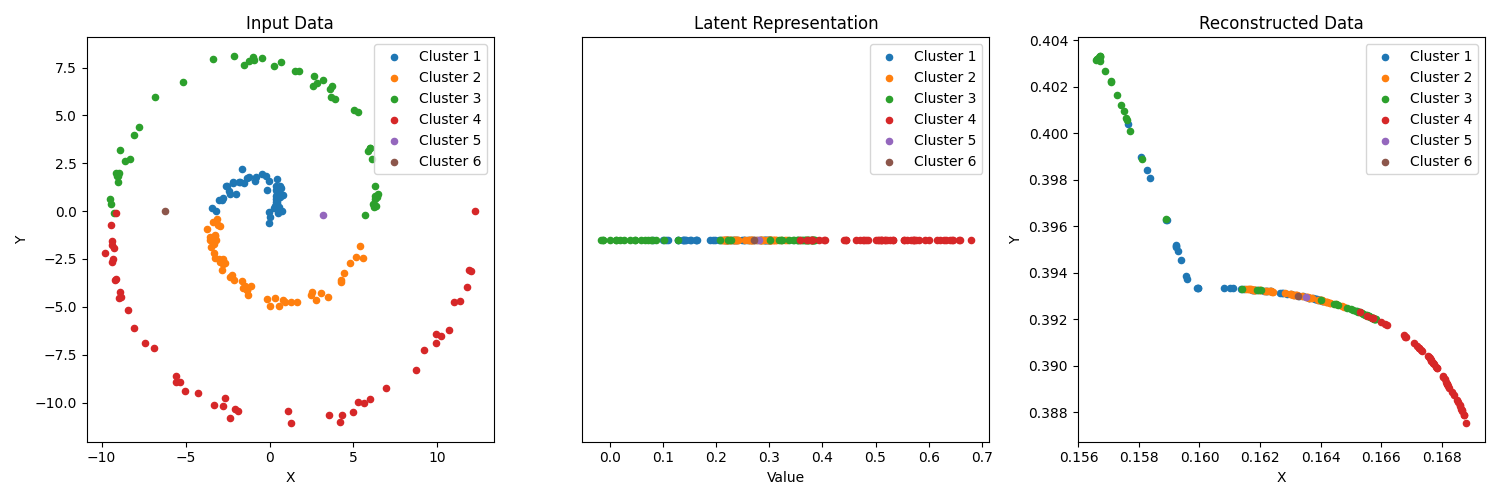
\includegraphics[width=\linewidth]{images/RQ2/tru/2DSwissRoll_64n_8k_3.7807.png}
    \caption{n=64, k=8 with 3.7807 softTW.}
    \label{fig:RQ2/tru/2DSwissRoll}
  \end{subfigure}

  \caption{Comparison of 2DSwissRoll dataset (202 instances) experiments with different unsupervised loss functions.}
  \label{fig:RQ2/2DSwissRoll}
\end{figure}

The \textbf{2DSwissRoll} (Dataset \ref{fig:2DSwissRoll}, Experiment \ref{fig:RQ2/2DSwissRoll}) dataset represents the most complex two-dimensional scenario within the experimental framework, and its evaluation highlights the limitations of the tested loss functions in handling highly non-linear manifold structures. Unlike the blob or moon datasets, which are composed of relatively simple clusters or arcs, the Swiss roll introduces a continuous spiral manifold segmented into colored sections, with IBIs deliberately positioned at the boundaries between these segments. The ideal outcome in the latent space would be an unfolded representation of the spiral, where the red section appears at one end, followed in sequence by green, yellow, and blue, with the IBIs faithfully placed at the transition zones between sections. This kind of unfolding would preserve both the global continuity of the manifold and the local transitional structure.

In practice, none of the examined losses achieved this expectation. MSE, while providing by far the strongest reconstruction, essentially reproduces the rolled manifold as it appears in the input space rather than unfolding it. The local and global geometry of the data is preserved well in reconstruction, and IBIs are placed in a manner consistent with their transitional nature. However, the lack of unfolding in the latent space indicates that the model has learned only to mimic the input geometry rather than transform it into a more interpretable lower-dimensional representation. This suggests that MSE alone is insufficient when the task requires revealing hidden manifold structure and that an additional objective explicitly encouraging unfolding would be necessary.

The other loss functions perform no better in this regard. Cosine similarity and Kullback–Leibler divergence both fail to generate a meaningful unfolding, and their reconstructions lose much of the structural fidelity observed with MSE. In both cases, the latent representations do not disentangle the sequential order of the manifold, and IBIs are not positioned with the clarity one would expect in a successful unfolding. The most promising candidate, based on its local neighborhood emphasis, was the soft trustworthiness loss. Because this loss embeds neighborhoods iteratively, there was an expectation that it might capture the local continuity of the spiral and gradually unroll it in latent space. Yet the results show that even soft trustworthiness was unable to unfold the Swiss roll. Its embeddings preserve some local neighborhood relationships, but this preservation does not translate into a meaningful global unrolling of the manifold.

The findings from the 2DSwissRoll dataset therefore underscore the limitations of the examined objectives when faced with complex manifold learning tasks. While MSE continues to demonstrate superior reconstruction fidelity, its inability to produce an unfolded latent representation highlights a gap that cannot be closed by simple reconstruction losses alone. Similarly, the failure of cosine similarity, KLD, and even soft trustworthiness to unfold the manifold indicates that objectives with purely local or distributional perspectives are insufficient in this context. This dataset makes clear that additional objectives specifically designed for manifold unfolding are required if such tasks are to be addressed effectively.

% 3DBlobsS
\begin{figure}[htbp]
  \centering
  % subfigure 1
  \begin{subfigure}[b]{1.0\textwidth}
    \centering
    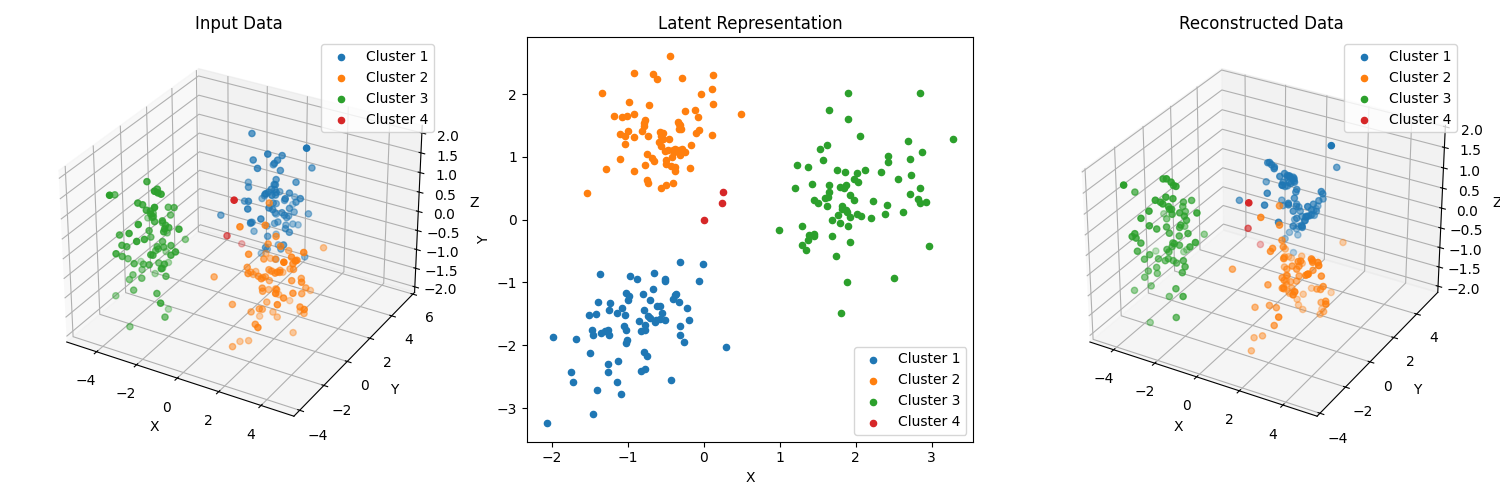
\includegraphics[width=\linewidth]{images/RQ2/mse/3DBlobsS_-1_0.0507.png}
    \caption{n=228 with 0.0507 MSE.}
    \label{fig:RQ2/mse/3DBlobsS}
  \end{subfigure}
  \hfill
  % subfigure 2
  \begin{subfigure}[b]{1.0\textwidth}
    \centering
    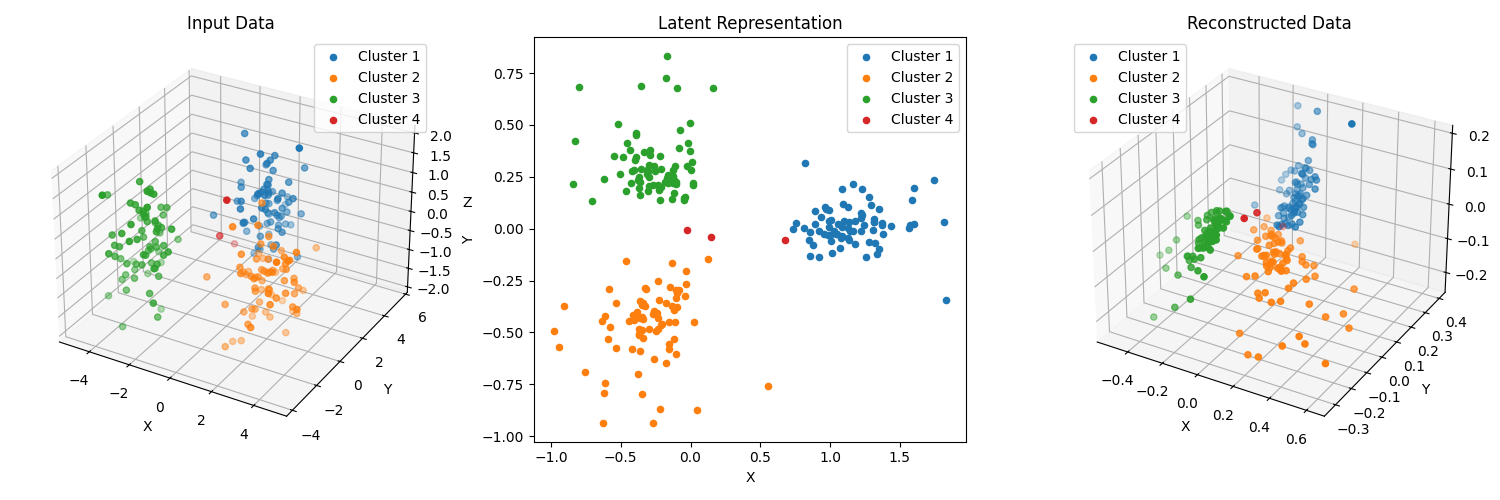
\includegraphics[width=\linewidth]{images/RQ2/csi/3DBlobsS_-1_0.0006.png}
    \caption{n=228 with 0.0006 CosSim.}
    \label{fig:RQ2/csi/3DBlobsS}
  \end{subfigure}
  \hfill
  % subfigure 3
  \begin{subfigure}[b]{1.0\textwidth}
    \centering
    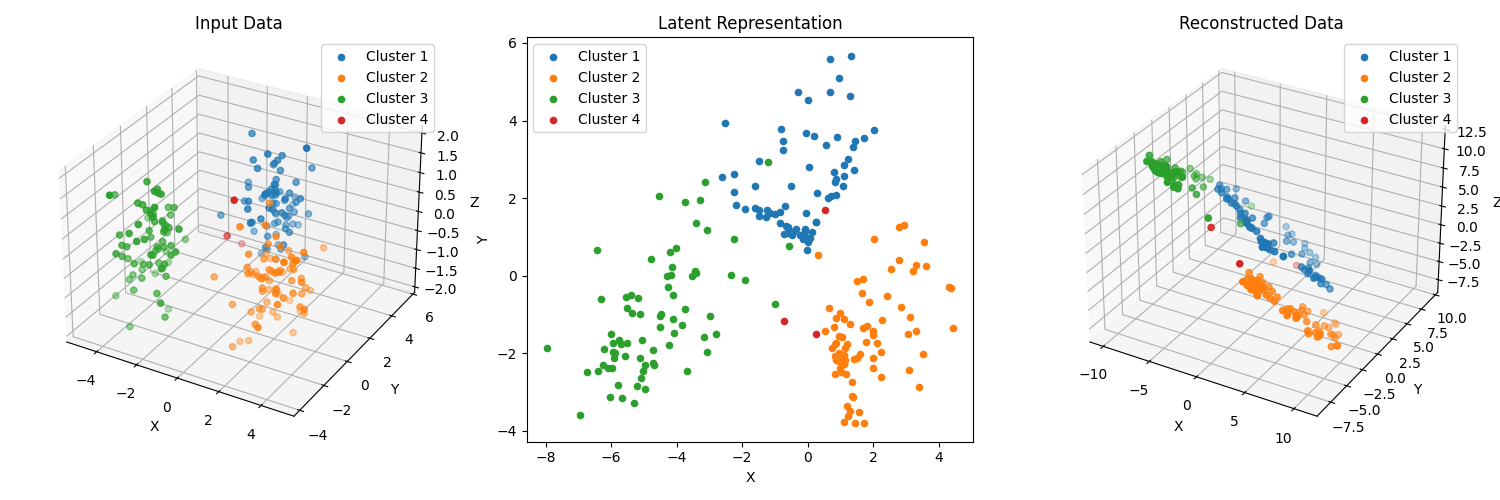
\includegraphics[width=\linewidth]{images/RQ2/kld/3DBlobsS_-1_0.0002.png}
    \caption{n=228 with 0.0002 KLD.}
    \label{fig:RQ2/kld/3DBlobsS}
  \end{subfigure}
  \hfill
  % subfigure 4
  \begin{subfigure}[b]{1.0\textwidth}
    \centering
    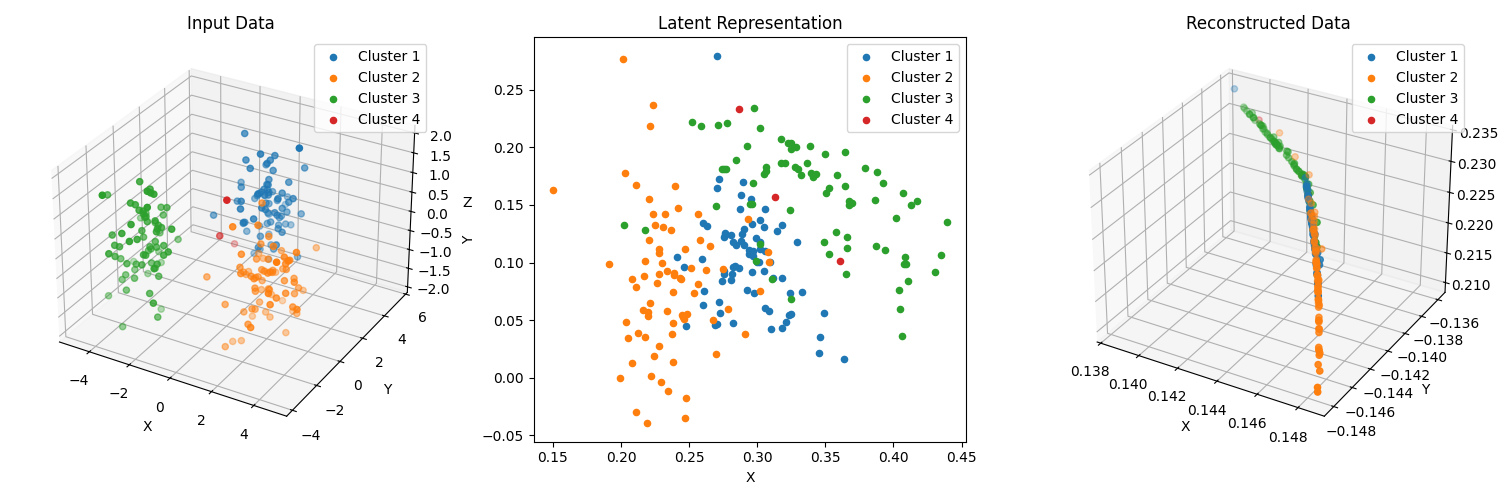
\includegraphics[width=\linewidth]{images/RQ2/tru/3DBlobsS_128n_8k_7.8846.png}
    \caption{n=128, k=8 with 7.8846 softTW.}
    \label{fig:RQ2/tru/3DBlobsS}
  \end{subfigure}

  \caption{Comparison of 3DBlobsS dataset (228 instances) experiments with different unsupervised loss functions.}
  \label{fig:RQ2/3DBlobsS}
\end{figure}

The \textbf{3DBlobsS} (Dataset \ref{fig:3DBlobsS}, Experiment \ref{fig:RQ2/3DBlobsS}) dataset can be understood as a straightforward extension of the earlier 2DBlobsS case into three dimensions. It consists of three compact Gaussian clusters with a small number of IBIs positioned in between them. This shift from two to three dimensions introduces an additional degree of representational freedom, while the autoencoder itself is constrained by a two-dimensional bottleneck. Consequently, one might expect the reconstructions to collapse naturally onto a two-dimensional manifold, reflecting the compression enforced by the architecture. Interestingly, the results reveal that this is not always the case, and that some loss functions are capable of maintaining genuinely three-dimensional reconstructions even after dimensionality reduction in the latent space.

MSE performs particularly well in this respect. In the latent space, the embedding is near perfect: clusters are clearly separated, and IBIs are positioned precisely in the transitional zones between them. The reconstructions preserve not only the cluster geometry but also the three-dimensional nature of the dataset. Despite the bottleneck constraint, the reconstruction does not reduce to a flat two-dimensional surface but instead retains volume, capturing the full structure of the input distribution. Cosine similarity produces very similar results, yielding a strong latent embedding and reconstructions that remain convincingly three-dimensional. While not as flawless as MSE, it nevertheless manages to preserve both global cluster structure and the bridging role of IBIs.

KLD, by contrast, fails to preserve this three-dimensional character. In the reconstruction space, the data collapses onto a two-dimensional manifold, which is consistent with the bottleneck compression but in this case, indicates a poor loss objective. This collapse is reflected in the latent embeddings, where cluster boundaries are weaker and IBIs are less distinctly separated than under MSE or cosine similarity. Although the clusters remain roughly identifiable and the IBIs are not entirely misplaced, the representation lacks the clarity observed in the stronger losses.

The weakest performance emerges from the soft trustworthiness objective. In this case, the reconstruction degenerates further, with the data collapsing onto a one-dimensional manifold. This simplification erases much of the dataset’s original structure and translates directly into a poor latent embedding. The clusters merge extensively, with little evidence of distinct boundaries, and the IBIs are no longer represented as transitional elements. Instead, they collapse into the green cluster, which undermines their interpretive value. This result highlights the tendency of soft trustworthiness to overemphasize local relationships at the cost of preserving global geometry, a trade-off that proves especially damaging in higher-dimensional cases.

Taken together, the results from 3DBlobsS reinforce the strong performance of MSE and cosine similarity, both of which are able to preserve the essential structure of the dataset in both latent and reconstruction space. KLD provides an acceptable but weakened representation, collapsing the data into a lower-dimensional form that reduces clarity while still preserving some degree of cluster separation. Soft trustworthiness, however, fails to maintain the dataset’s structural integrity, producing reconstructions and embeddings that obscure both cluster identity and the role of IBIs. This dataset therefore illustrates that, even when moving into higher-dimensional input spaces, the hierarchy of loss function performance remains consistent, with MSE providing the most faithful balance of reconstruction and embedding quality.

% 3DBlobsM
\begin{figure}[htbp]
  \centering
  % subfigure 1
  \begin{subfigure}[b]{1.0\textwidth}
    \centering
    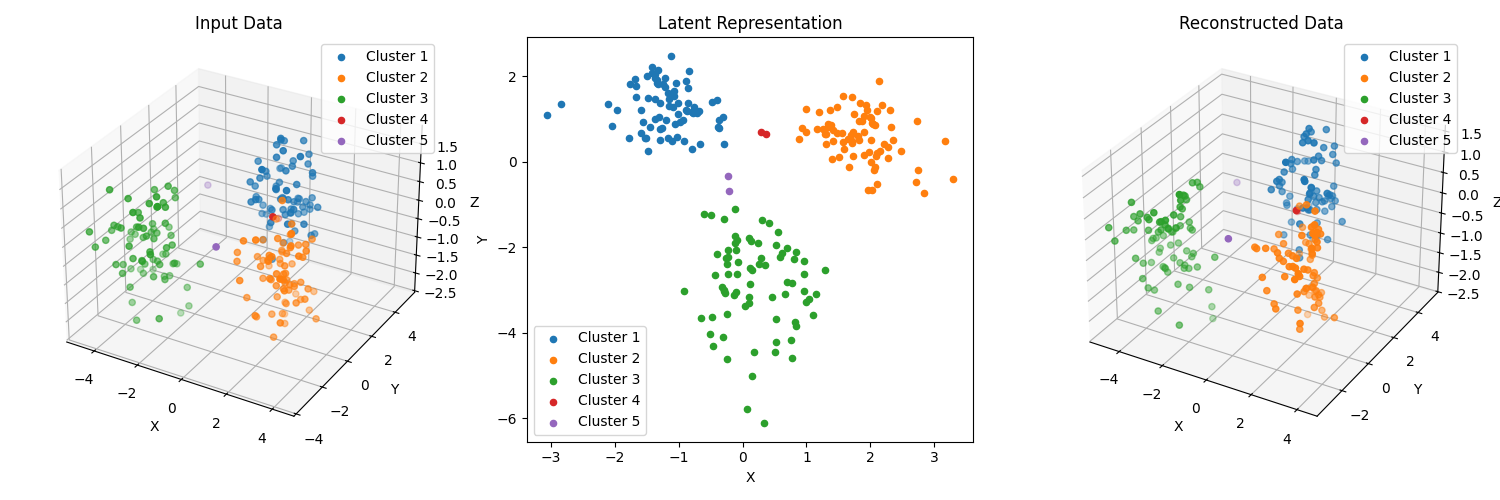
\includegraphics[width=\linewidth]{images/RQ2/mse/3DBlobsM_-1_0.0443.png}
    \caption{n=229 with 0.0443 MSE.}
    \label{fig:RQ2/mse/3DBlobsM}
  \end{subfigure}
  \hfill
  % subfigure 2
  \begin{subfigure}[b]{1.0\textwidth}
    \centering
    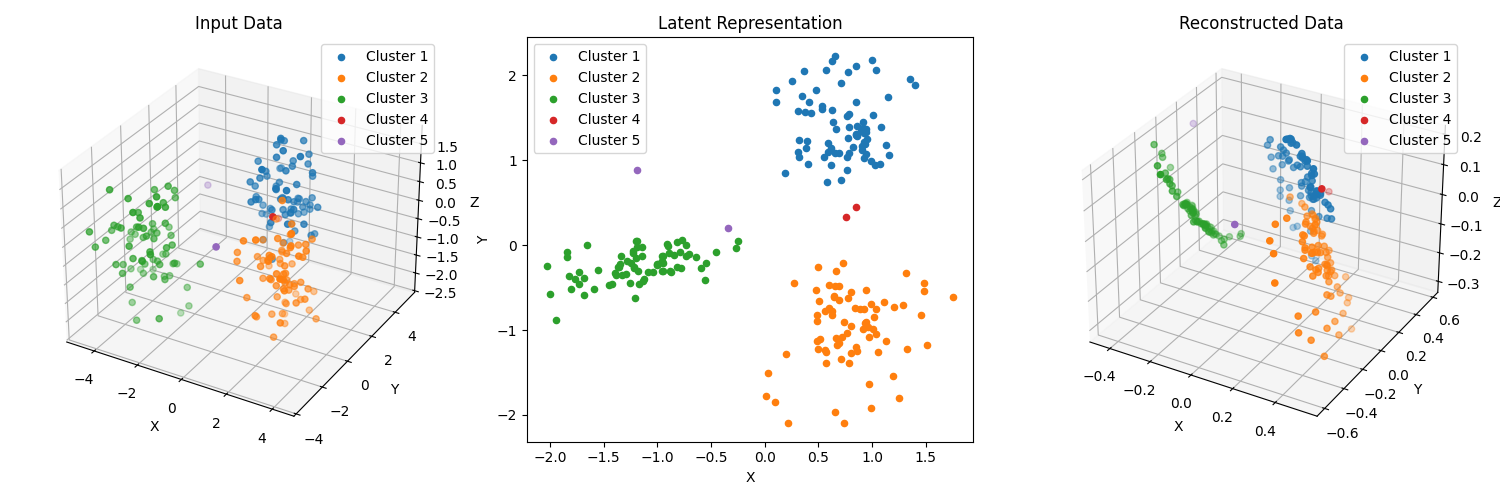
\includegraphics[width=\linewidth]{images/RQ2/csi/3DBlobsM_-1_0.0003.png}
    \caption{n=229 with 0.0003 CosSim.}
    \label{fig:RQ2/csi/3DBlobsM}
  \end{subfigure}
  \hfill
  % subfigure 3
  \begin{subfigure}[b]{1.0\textwidth}
    \centering
    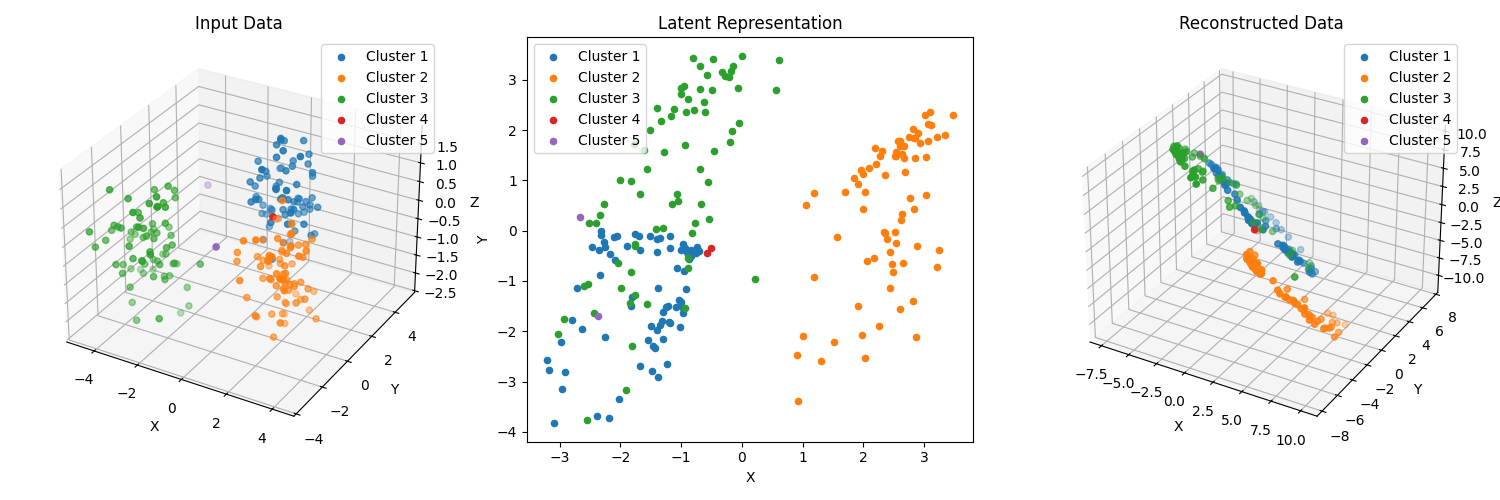
\includegraphics[width=\linewidth]{images/RQ2/kld/3DBlobsM_-1_0.0002.png}
    \caption{n=229 with 0.0002 KLD.}
    \label{fig:RQ2/kld/3DBlobsM}
  \end{subfigure}
  \hfill
  % subfigure 4
  \begin{subfigure}[b]{1.0\textwidth}
    \centering
    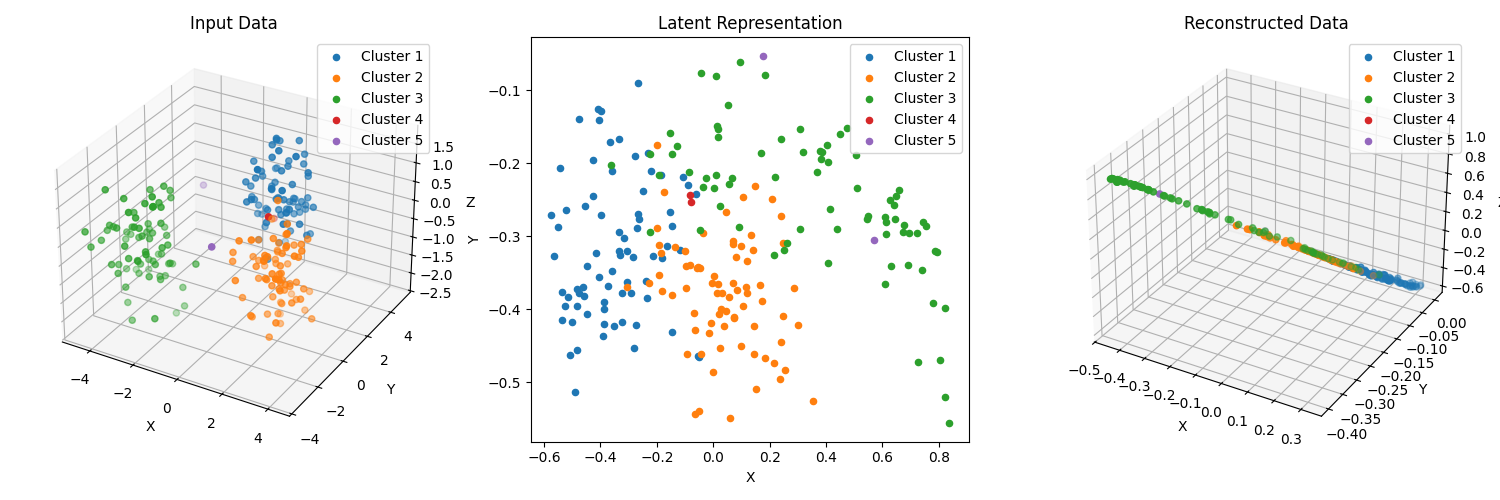
\includegraphics[width=\linewidth]{images/RQ2/tru/3DBlobsM_128n_8k_7.8841.png}
    \caption{n=128, k=8 with 7.8841 softTW.}
    \label{fig:RQ2/tru/3DBlobsM}
  \end{subfigure}

  \caption{Comparison of 3DBlobsM dataset (229 instances) experiments with different unsupervised loss functions.}
  \label{fig:RQ2/3DBlobsM}
\end{figure}

The \textbf{3DBlobsM} (Dataset \ref{fig:3DBlobsM}, Experiment \ref{fig:RQ2/3DBlobsM}) dataset extends the 3DBlobsS case by introducing a more challenging configuration of clusters and IBIs. While the overall setup remains similar, with three Gaussian clusters and transitional instances placed between them, the geometry of the IBIs is more complex, as two separate sets of transitional points are introduced. This makes the evaluation of embeddings and reconstructions more difficult, particularly when assessing which loss function represents the IBIs most faithfully. In fact, one limitation in this analysis stems from the orientation of the original dataset itself, which does not always allow for a straightforward judgment of which embedding corresponds more closely to the ground truth transitional relationships.

As in the simpler 3DBlobsS case, MSE and cosine similarity once again deliver very strong results. The latent embeddings clearly separate the clusters, and IBIs occupy transitional positions. However, the placement of the purple IBIs differs between the two losses, and it is not possible to determine retrospectively which representation is more faithful to the true underlying distribution. This ambiguity underscores the difficulty of visually evaluating high-dimensional transitional structures when the original orientation complicates interpretation. Still, both losses reconstruct the dataset convincingly and maintain the three-dimensional nature of the data despite the bottleneck compression.

KLD shows weaker performance. In this case, the blue and green clusters merge together in both latent and reconstruction space, resulting in a significant loss of structural clarity. The red IBIs are placed acceptably, positioned near the boundary between clusters, but the purple IBIs are embedded poorly. One of them ends up absorbed into the merged blue–green cluster, undermining its role as a transitional point. This once again illustrates the tendency of KLD to collapse cluster boundaries, a behavior that compromises both reconstruction quality and IBI fidelity.

The soft trustworthiness loss also produces merged clusters, but in this case the outcome is less arbitrary than with KLD. Rather than collapsing specific clusters together, soft trustworthiness results in all clusters taking up the same space in a way that reflects their relative size relationships fairly well. This outcome demonstrates the strength of the objective’s local-neighborhood perspective, which ensures that internal cluster structure is captured more faithfully than in the KLD case. However, the treatment of IBIs remains problematic. Instead of being placed in meaningful transitional positions, the IBIs appear scattered across the embedding, with no clear bridging function preserved. Thus, while the clusters themselves are represented with a degree of fidelity under soft trustworthiness, the IBIs lose their interpretive value.

In summary, the 3DBlobsM dataset reinforces the patterns already observed in 3DBlobsS. MSE and cosine similarity consistently provide strong embeddings and reconstructions, though subtle differences in IBI placement remain difficult to interpret due to dataset orientation. KLD demonstrates the weakness of its distributional approach by collapsing clusters and misplacing IBIs, while soft trustworthiness, although somewhat successful at embedding cluster structures consistently, fails to provide meaningful representations of transitional points. The dataset thereby highlights both the reliability of MSE and cosine similarity for global structure preservation and the limitations of the more specialized objectives when applied to complex three-dimensional transitions.

% 3DMoons
\begin{figure}[htbp]
  \centering
  % subfigure 1
  \begin{subfigure}[b]{1.0\textwidth}
    \centering
    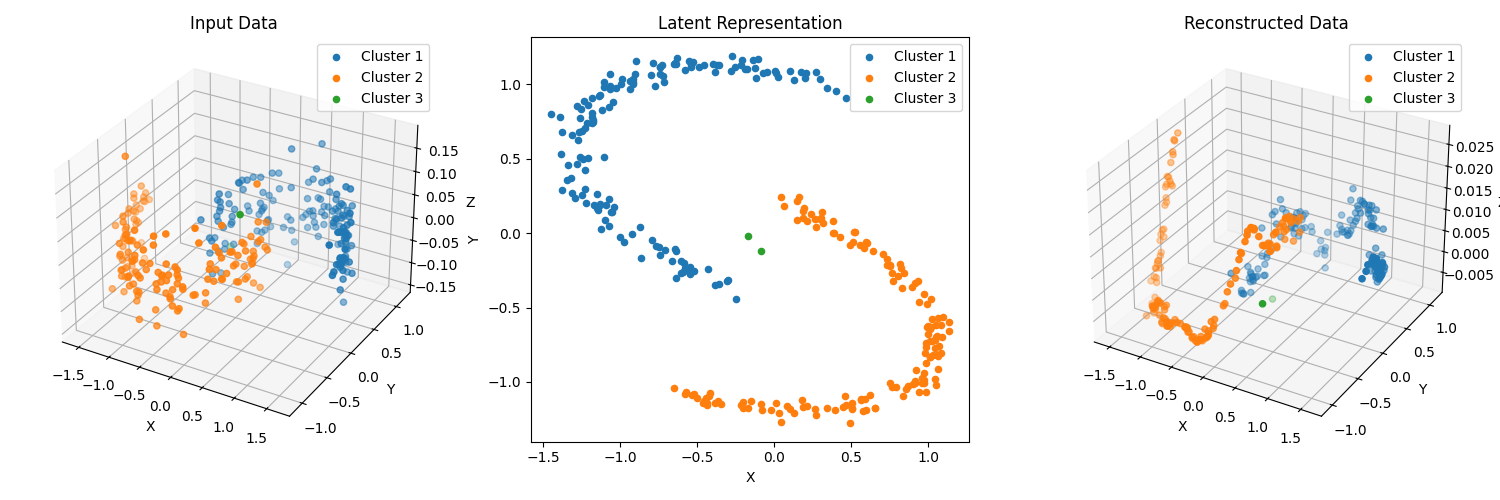
\includegraphics[width=\linewidth]{images/RQ2/mse/3DMoons_-1_0.0008.png}
    \caption{n=302 with 0.0008 MSE.}
    \label{fig:RQ2/mse/3DMoons}
  \end{subfigure}
  \hfill
  % subfigure 2
  \begin{subfigure}[b]{1.0\textwidth}
    \centering
    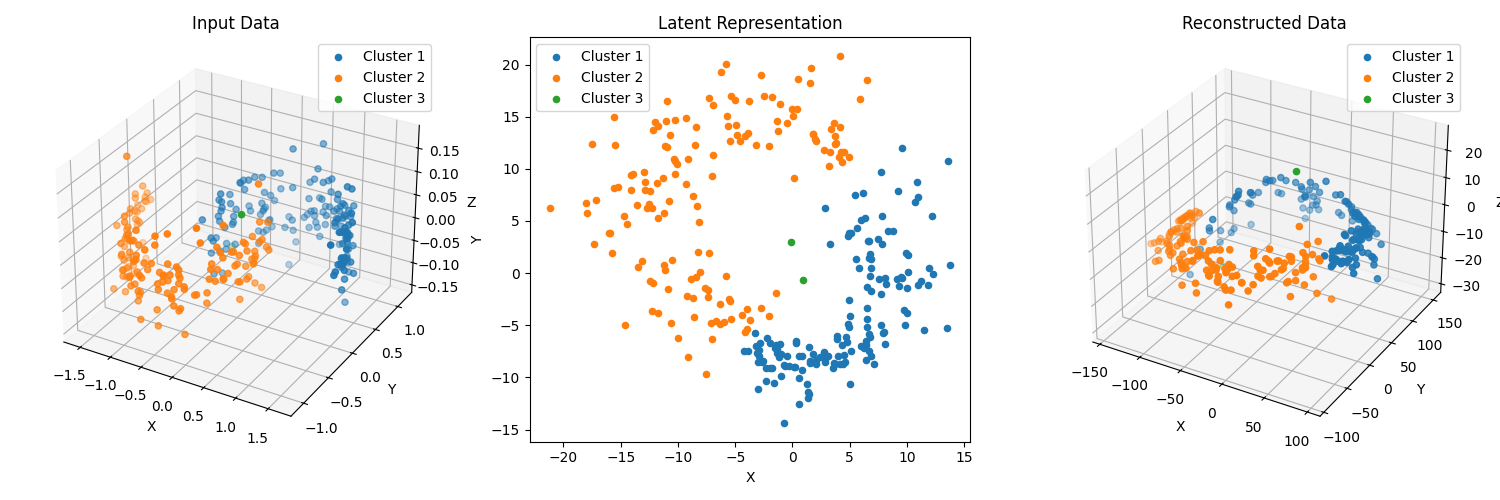
\includegraphics[width=\linewidth]{images/RQ2/csi/3DMoons_2_0.0002.png}
    \caption{n=302 with 0.0002 CosSim.}
    \label{fig:RQ2/csi/3DMoons}
  \end{subfigure}
  \hfill
  % subfigure 3
  \begin{subfigure}[b]{1.0\textwidth}
    \centering
    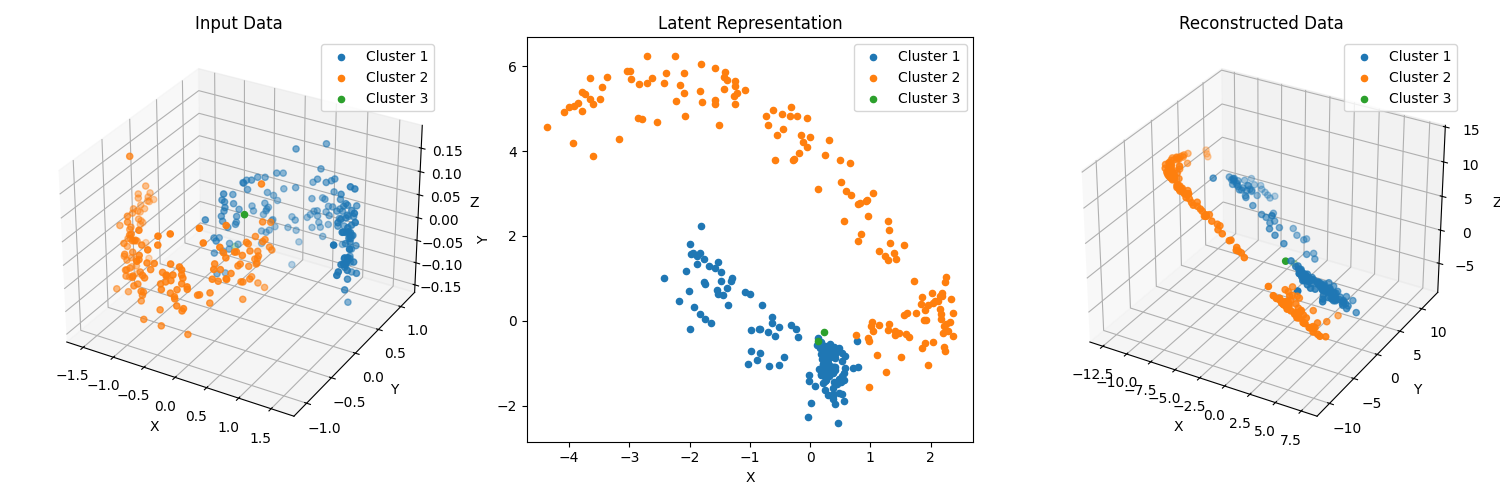
\includegraphics[width=\linewidth]{images/RQ2/kld/3DMoons_-1_0.0005.png}
    \caption{n=302 with 0.0005 KLD.}
    \label{fig:RQ2/kld/3DMoons}
  \end{subfigure}
  \hfill
  % subfigure 4
  \begin{subfigure}[b]{1.0\textwidth}
    \centering
    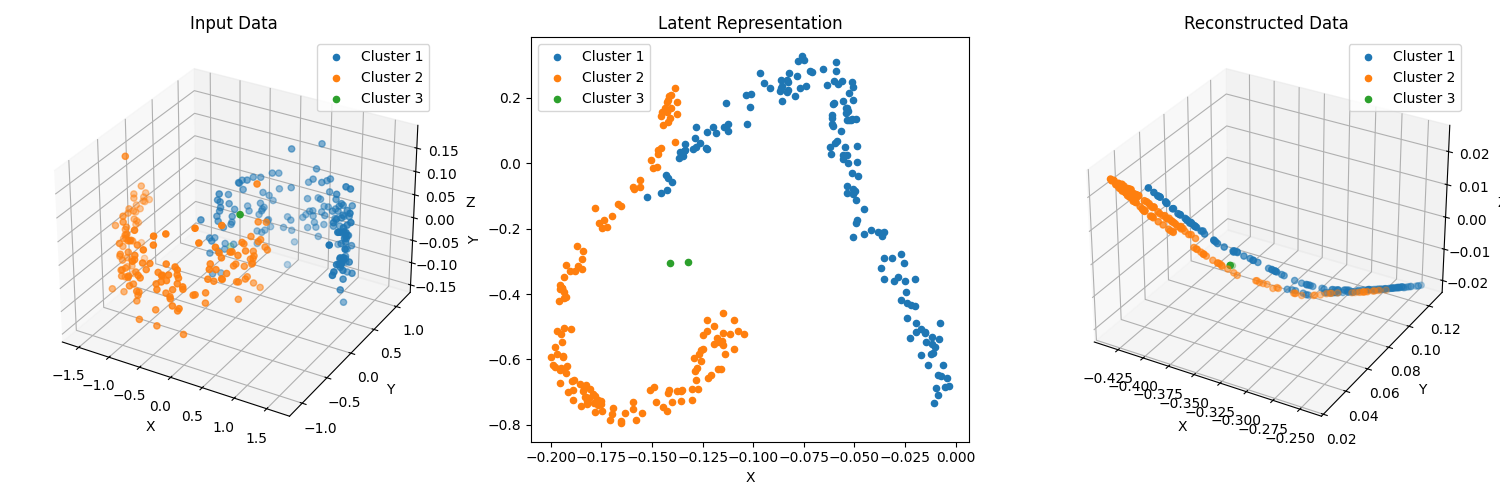
\includegraphics[width=\linewidth]{images/RQ2/tru/3DMoons_128n_16k_3.7874.png}
    \caption{n=128, k=16 with 3.7874 softTW.}
    \label{fig:RQ2/tru/3DMoons}
  \end{subfigure}

  \caption{Comparison of 3DMoons dataset (302 instances) experiments with different unsupervised loss functions.}
  \label{fig:RQ2/3DMoons}
\end{figure}

The \textbf{3DMoons} (Dataset \ref{fig:3DMoons}, Experiment \ref{fig:RQ2/3DMoons}) dataset is a direct extension of the 2DMoons configuration into three dimensions, retaining the same crescent-like clusters but introducing an additional degree of freedom in space. This added dimensionality increases the difficulty of reconstruction, since the model must now preserve both the curved structure of the moons and their skewed placement relative to one another, all while passing through a two-dimensional bottleneck. As with earlier cases, this dataset provides an opportunity to evaluate how well the different loss functions capture both the global shape of the moons and the transitional role of the IBIs under greater structural complexity.

MSE provides the strongest latent embedding, even though its reconstructions do not look particularly promising. The moons’ general form is preserved in the latent space with a level of fidelity that can reasonably be considered the best achievable given the bottleneck constraint. While finer details such as the precise width of the moons are not retained, the global arrangement of the arcs is convincing, and the IBIs are positioned in a way that reflects their bridging role. This underscores the capacity of MSE to generate embeddings that remain interpretable despite reconstruction weaknesses, and it aligns with earlier observations that this loss produces the most reliable low-dimensional representations overall.

Cosine similarity performs less convincingly. In this case, the information about the skewed placement of the two moons is lost, and the representation simplifies them into more centrally positioned, thickened structures. The IBIs are embedded centrally between these collapsed moons, but this placement reflects the loss of structural information rather than a faithful preservation of the data’s transitional points. The width and spatial offset of the moons, which are crucial for the dataset’s geometry, are therefore not captured.

KLD and soft trustworthiness also yield suboptimal representations. Under KLD, some parts of the blue cluster collapse, and the symmetry of the moons is disrupted. The IBIs end up embedded within the boundaries of these collapsed arcs, which weakens their interpretive value as transitional instances. The latent representation fails to preserve either the curvature or the separation of the moons, continuing the pattern observed in earlier datasets where KLD tends to reduce structural clarity. Soft trustworthiness performs somewhat better in this respect. While it too struggles to preserve the full structure of the moons, its local-neighborhood focus allows it to represent parts of the dataset more faithfully, particularly in the yellow cluster. As a result, the IBIs are placed relatively well within this context, even though the broader structure of the moons remains distorted.

Taken together, the 3DMoons results reaffirm the hierarchy observed in the two-dimensional version of the dataset. MSE produces the strongest latent embeddings, preserving global structure as effectively as possible under the bottleneck limitation, even if the reconstructions remain imperfect. Cosine similarity loses key geometric features such as skew and width, and both KLD and soft trustworthiness struggle with the symmetry and separation of the moons. Of these, soft trustworthiness yields the more coherent treatment of IBIs, but still falls short of a globally faithful embedding. The dataset therefore underscores both the strengths of MSE in generating usable embeddings and the persistent weaknesses of the alternative losses when faced with non-linear cluster geometries in higher dimensions.

% 3DSwissRoll
\begin{figure}[htbp]
  \centering
  % subfigure 1
  \begin{subfigure}[b]{1.0\textwidth}
    \centering
    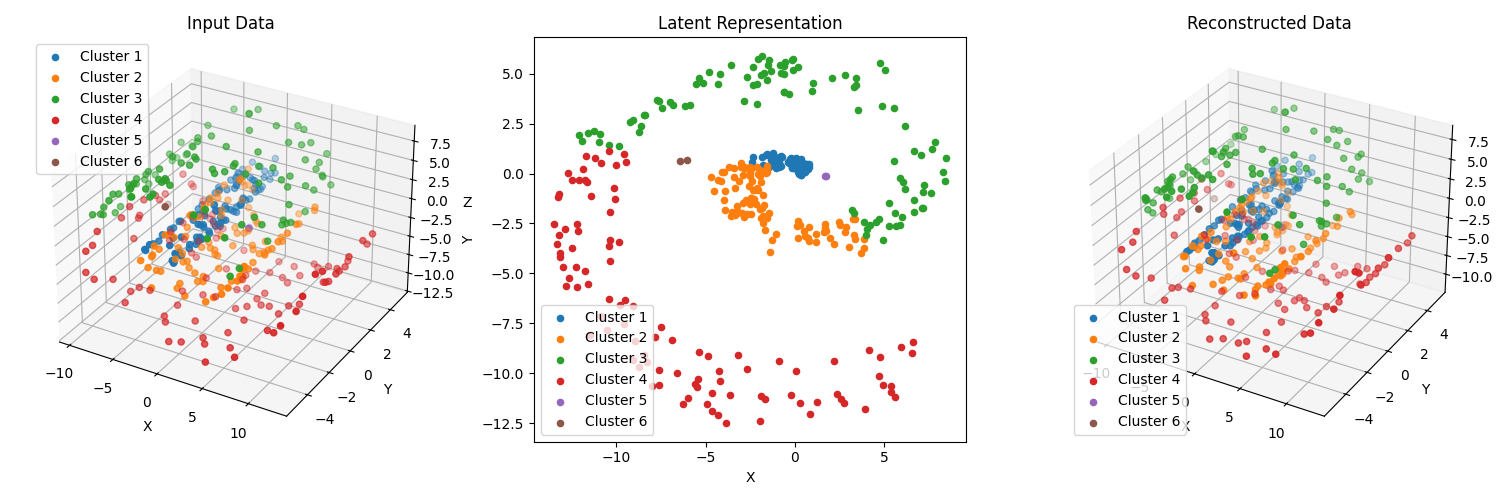
\includegraphics[width=\linewidth]{images/RQ2/mse/3DSwissRoll_-1_0.0487.png}
    \caption{n=404 with 0.0487 MSE.}
    \label{fig:RQ2/mse/3DSwissRoll}
  \end{subfigure}
  \hfill
  % subfigure 2
  \begin{subfigure}[b]{1.0\textwidth}
    \centering
    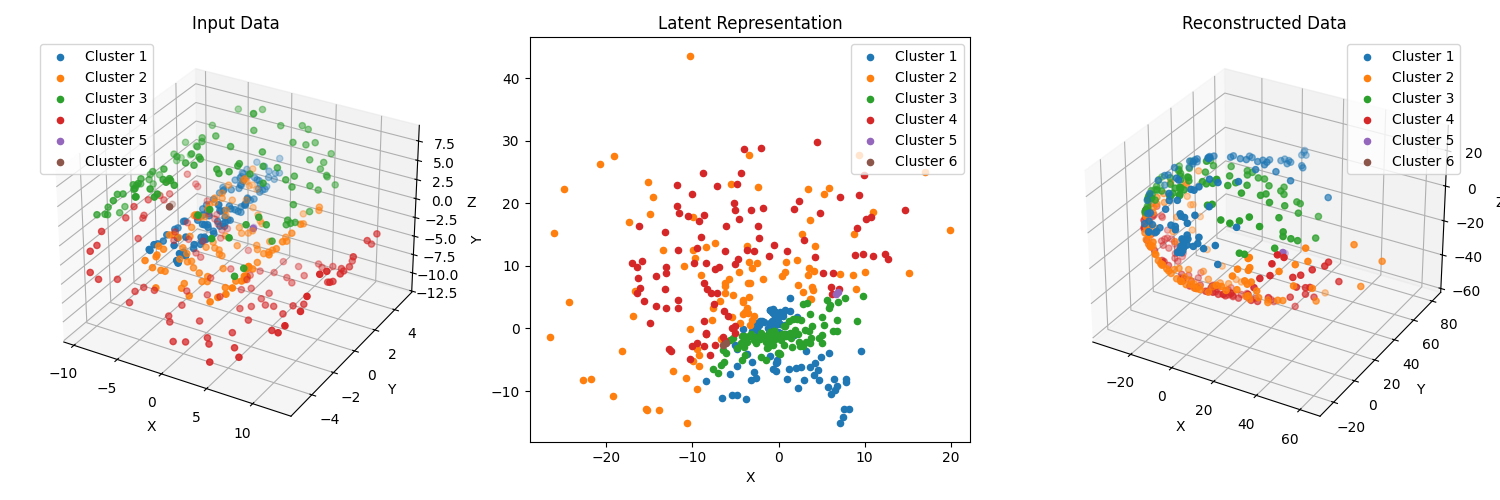
\includegraphics[width=\linewidth]{images/RQ2/csi/3DSwissRoll_2_0.0010.png}
    \caption{n=404 with 0.0010 CosSim.}
    \label{fig:RQ2/csi/3DSwissRoll}
  \end{subfigure}
  \hfill
  % subfigure 3
  \begin{subfigure}[b]{1.0\textwidth}
    \centering
    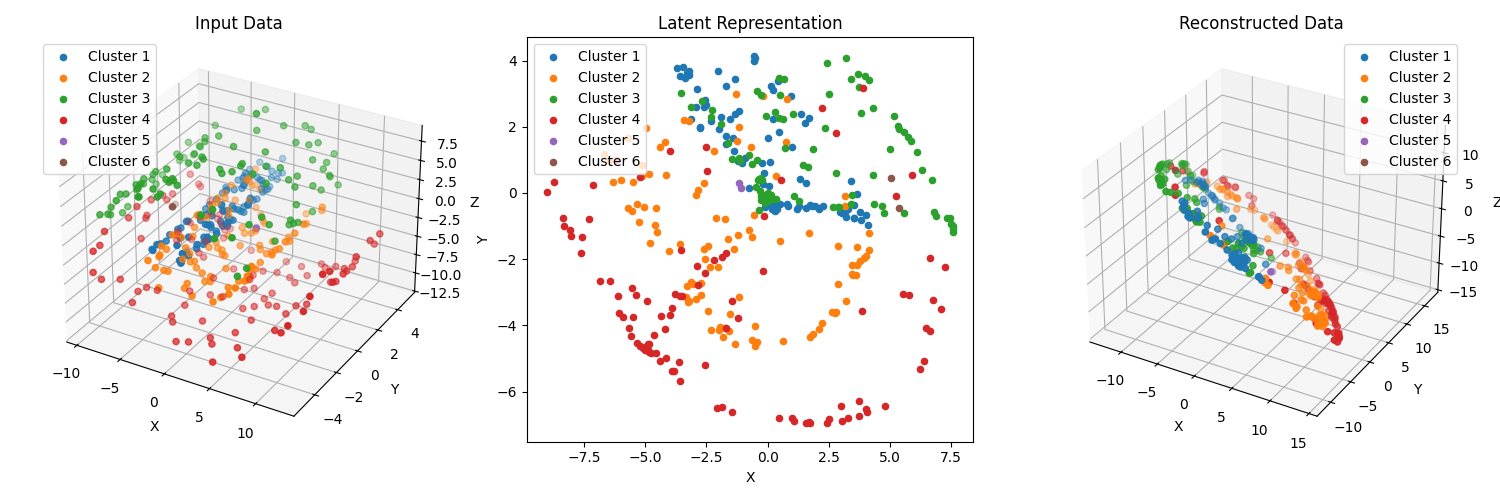
\includegraphics[width=\linewidth]{images/RQ2/kld/3DSwissRoll_-1_0.0005.png}
    \caption{n=404 with 0.0005 KLD.}
    \label{fig:RQ2/kld/3DSwissRoll}
  \end{subfigure}
  \hfill
  % subfigure 4
  \begin{subfigure}[b]{1.0\textwidth}
    \centering
    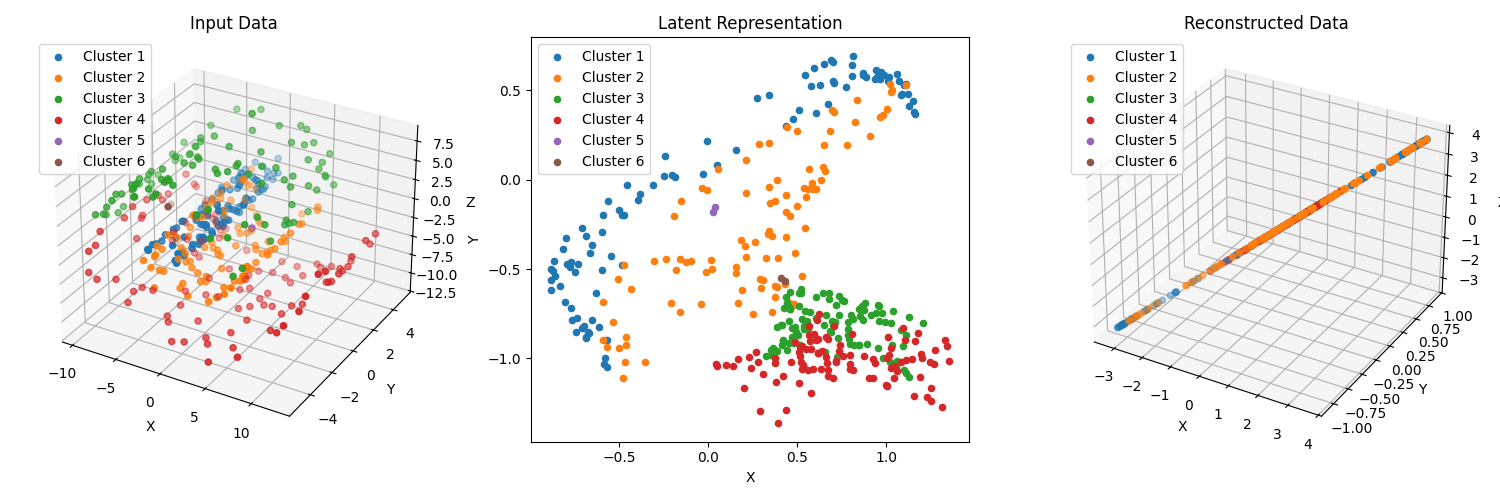
\includegraphics[width=\linewidth]{images/RQ2/tru/3DSwissRoll_256n_16k_7.5884.png}
    \caption{n=256, k=16 with 7.5884 softTW.}
    \label{fig:RQ2/tru/3DSwissRoll}
  \end{subfigure}

  \caption{Comparison of 3DSwissRoll dataset (404 instances) experiments with different unsupervised loss functions.}
  \label{fig:RQ2/3DSwissRoll}
\end{figure}

The \textbf{3DSwissRoll} (Dataset \ref{fig:3DSwissRoll}, Experiment \ref{fig:RQ2/3DSwissRoll}) dataset extends the challenge of the 2DSwissRoll into three dimensions, thereby increasing both the complexity of the manifold structure and the demands placed on the reconstruction and embedding objectives. As before, the task is not simply to preserve the rolled geometry of the data but ideally to achieve an unfolding of the manifold in latent space, such that the colored sections appear in the correct sequence, red followed by green, yellow, and blue, with IBIs faithfully positioned at the boundaries between these regions. This goal provides a stringent test of the ability of the different loss functions to move beyond reconstruction fidelity toward meaningful manifold learning.

MSE once again demonstrates robust performance, both in reconstruction and in the latent embedding. The Swiss roll is represented faithfully, with the manifold preserved and IBIs positioned consistently with their transitional role. However, as in the two-dimensional case, MSE does not succeed in unrolling the manifold. The spiral structure remains intact, which reflects a strength in terms of reconstruction fidelity but a limitation when the task requires a transformation into a more interpretable latent representation. In other words, MSE preserves the geometry of the input well but does not reorganize it into the simplified unfolded form that would best reveal the underlying data structure.

The most notable and promising result arises from the soft trustworthiness objective. While its reconstruction collapses onto a one-dimensional manifold in which little of the original structure is visible, the latent representation reveals that the Swiss roll has been partially unrolled. The unfolding is not complete, but it demonstrates the potential of this objective to capture the sequential relationships embedded in the manifold. Specifically, the embedding shows that the manifold narrows toward the center, where the brown IBIs are located, suggesting that the loss is capable of preserving both local neighborhoods and the transitional role of IBIs in a way that supports unrolling. However, the expected narrowing at the location of the purple IBIs does not occur, and the size of the sequences is not embedded faithfully. This shortcoming leads to the interpretation that while soft trustworthiness has the potential to achieve a smooth unrolling of the Swiss roll, the presence of IBIs may disrupt this process. It is plausible that in the absence of IBIs, the manifold could have been unfolded more consistently, pointing to both the strengths and the sensitivities of this loss.

Cosine similarity and KLD perform less convincingly. Neither manages to capture the roll structure in a meaningful way, and their embeddings fail to show signs of a coherent unrolling. The representation under KLD does, however, exhibit faint traces of structure that resemble a projection into a compound dimension, suggesting that some aspects of the manifold’s continuity are retained, albeit in a distorted form. Cosine similarity, by contrast, produces a poor embedding with little evidence of the roll’s sequential organization.

In summary, the 3DSwissRoll dataset illustrates the relative strengths and limitations of the different loss functions in particularly sharp relief. MSE remains the most reliable for faithful reconstruction, but it does not advance the further-reaching goal of unrolling the manifold. Soft trustworthiness emerges as the only loss to show signs of achieving this unrolling in the latent space, though its reconstruction collapses and its embedding remains incomplete. The fact that IBIs may interfere with this unfolding process is an important observation, suggesting that their inclusion can complicate manifold learning under local neighborhood–based objectives. Cosine similarity and KLD, meanwhile, fail to provide meaningful embeddings in this context, continuing their weaker performance relative to MSE. The results here therefore highlight both the stability of MSE as a baseline and the exploratory potential of soft trustworthiness for complex manifold unfolding, even if its current implementation does not fully succeed.

% 3DTorus
\begin{figure}[htbp]
  \centering
  % subfigure 1
  \begin{subfigure}[b]{1.0\textwidth}
    \centering
    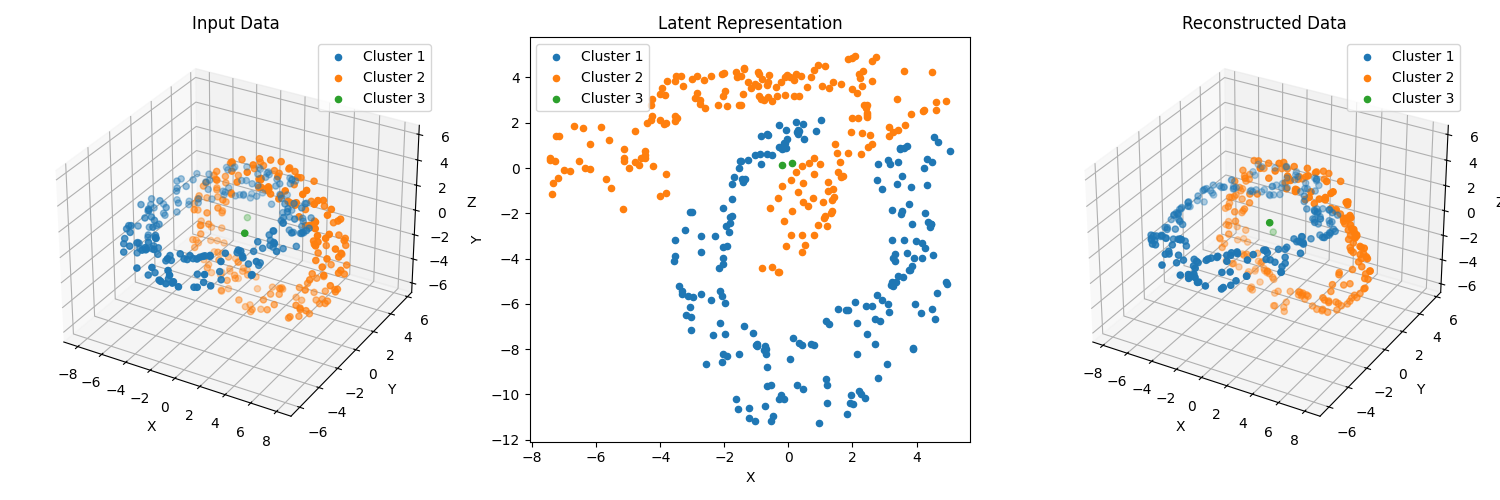
\includegraphics[width=\linewidth]{images/RQ2/mse/3DTorus_-1_0.0871.png}
    \caption{n=402 with 0.0871 MSE.}
    \label{fig:RQ2/mse/3DTorus}
  \end{subfigure}
  \hfill
  % subfigure 2
  \begin{subfigure}[b]{1.0\textwidth}
    \centering
    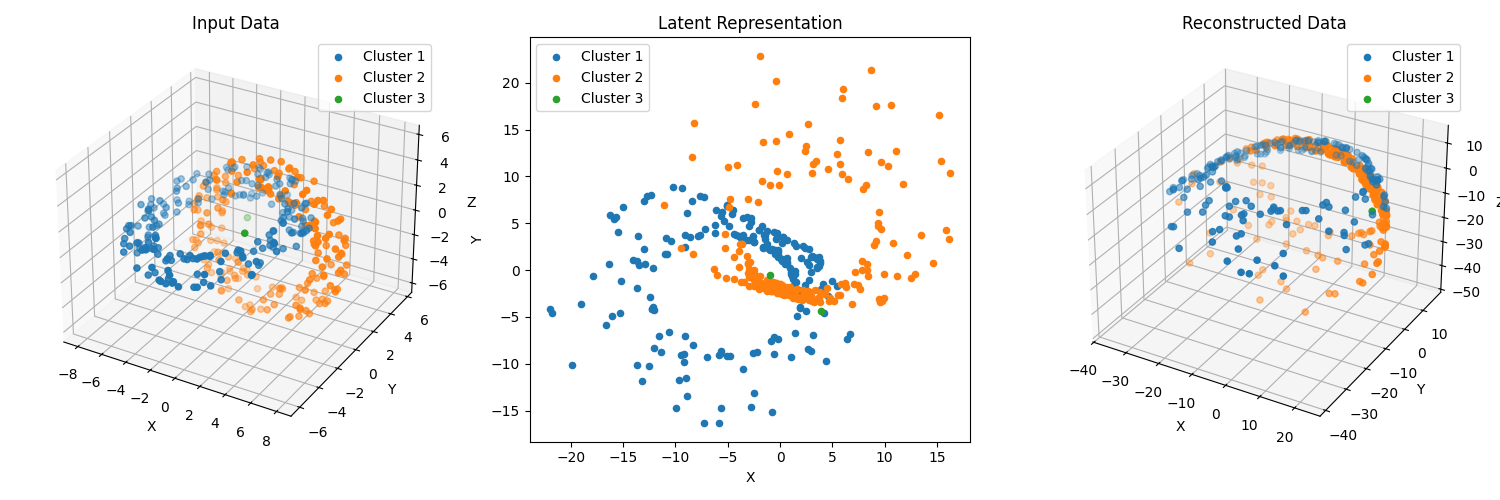
\includegraphics[width=\linewidth]{images/RQ2/csi/3DTorus_2_0.0006.png}
    \caption{n=402 with 0.0006 CosSim.}
    \label{fig:RQ2/csi/3DTorus}
  \end{subfigure}
  \hfill
  % subfigure 3
  \begin{subfigure}[b]{1.0\textwidth}
    \centering
    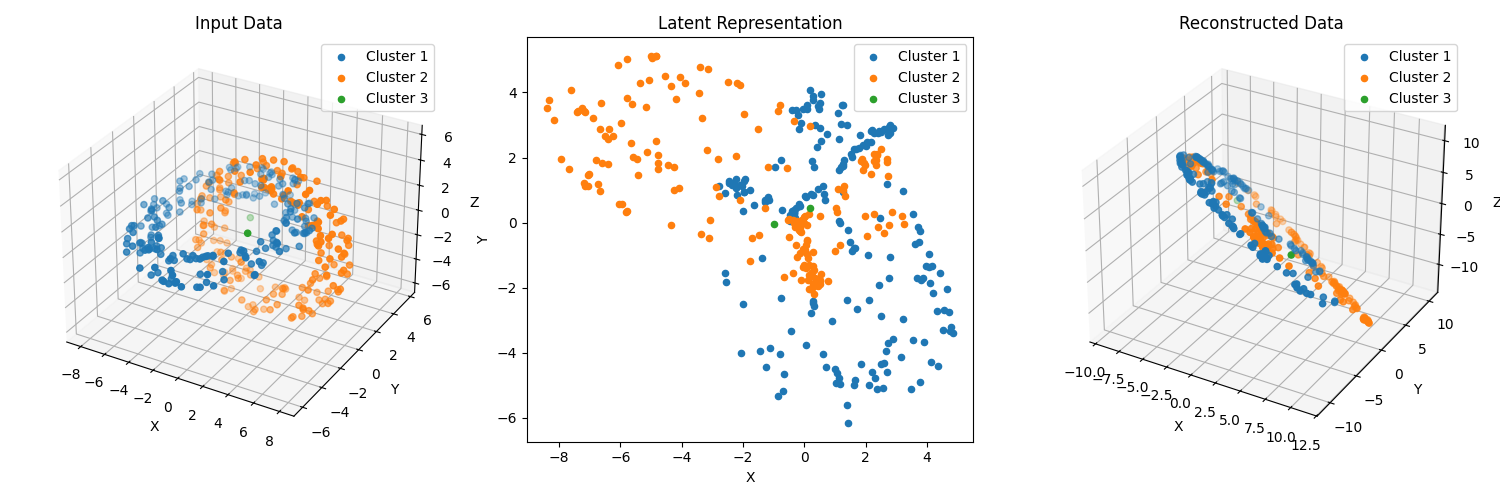
\includegraphics[width=\linewidth]{images/RQ2/kld/3DTorus_-1_0.0007.png}
    \caption{n=402 with 0.0007 KLD.}
    \label{fig:RQ2/kld/3DTorus}
  \end{subfigure}
  \hfill
  % subfigure 4
  \begin{subfigure}[b]{1.0\textwidth}
    \centering
    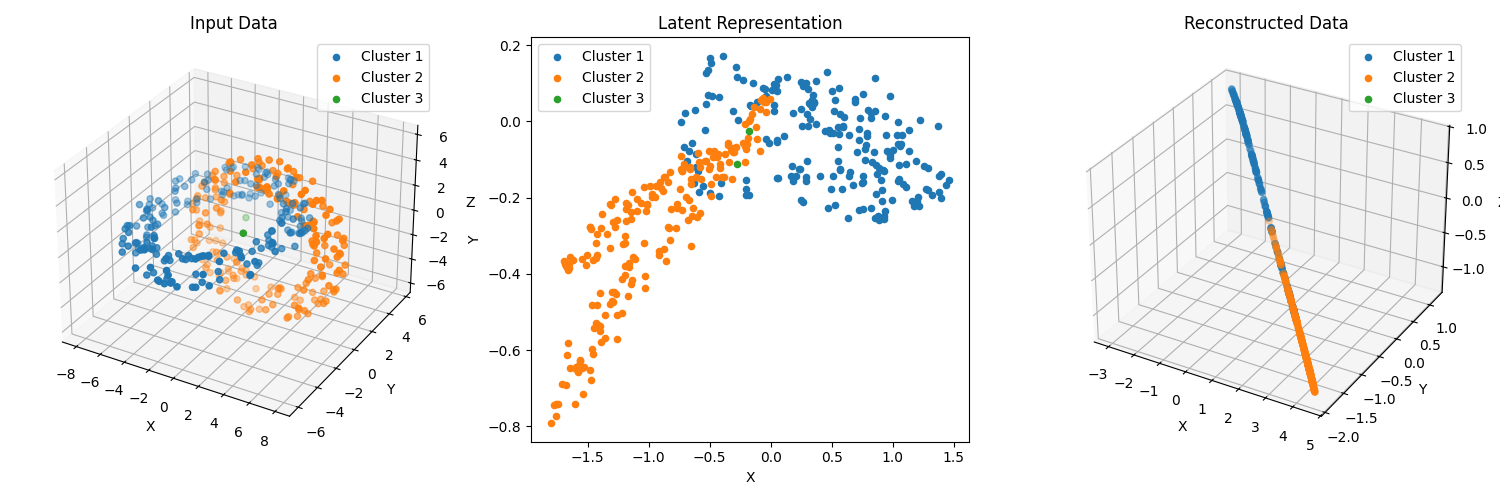
\includegraphics[width=\linewidth]{images/RQ2/tru/3DTorus_256n_16k_7.6641.png}
    \caption{n=256, k=16 with 7.6641 softTW.}
    \label{fig:RQ2/tru/3DTorus}
  \end{subfigure}

  \caption{Comparison of 3DTorus dataset (402 instances) experiments with different unsupervised loss functions.}
  \label{fig:RQ2/3DTorus}
\end{figure}

The \textbf{3DTorus} (Dataset \ref{fig:3DTorus}, Experiment \ref{fig:RQ2/3DTorus}) dataset is particularly interesting because it introduces a highly non-linear and intertwined cluster structure. Unlike the blob or moon datasets, where clusters are either compact or gently curved, the torus configuration consists of two ring-shaped manifolds that pass through one another in three-dimensional space. This creates a demanding scenario in which the objective is not only to preserve the integrity of each torus but also to represent their interwoven geometry in such a way that the IBIs appear naturally in the space between them. The dataset therefore provides a stringent test of whether the different loss functions are able to disentangle complex global structures while maintaining transitional fidelity.

MSE once again delivers the most convincing result. In the reconstruction space, the two tori are represented with striking accuracy, and the model even succeeds in “ripping” them apart in the latent space so that one can pass through the other without intersecting. This reorganization avoids the unrealistic overlap that might otherwise occur and results in a near-perfect reconstruction of the dataset’s global structure. The IBIs are also placed very well: they appear exactly in the middle of the two tori, reflecting their intended transitional role with high fidelity. This outcome demonstrates that MSE is not only capable of preserving local geometry but can also restructure global relationships in a way that avoids overlap, an ability that makes it uniquely suited to this type of data.

Cosine similarity performs less effectively. In this case, the two tori remain interwoven, but they are projected into a two-dimensional form where they overlap. This overlap introduces distortions that undermine the clarity of the structure, and it prevents the separation that is achieved under MSE. The IBIs reflect this partial failure: while one of them is embedded correctly, positioned in the transitional space between the tori, the other is misplaced, highlighting the inconsistency of the representation.

KLD and soft trustworthiness both yield weaker outcomes. In their latent embeddings, the torus structure is difficult to identify, suggesting that the global geometry of the data has been partly lost. This loss of structure undermines the interpretability of the embeddings and indicates that neither objective is well suited to capturing such complex intertwined manifolds. Nevertheless, the placement of IBIs under these losses is somewhat better than might be expected given the poor preservation of structure. The IBIs appear in locations that could reasonably be interpreted as transitional zones, even though the clusters themselves are distorted and overlapping. This indicates that both KLD and soft trustworthiness retain some capacity to reflect in-between relationships, albeit in a context where the underlying manifolds have not been faithfully preserved.

Overall, the results from the 3DTorus dataset highlight both the strengths and the limitations of the tested objectives in handling highly non-linear and intertwined structures. MSE stands out as the only loss capable of producing a near-perfect reconstruction and an embedding that avoids overlap while positioning the IBIs with high accuracy. Cosine similarity retains some features of the torus structure but fails to disentangle the manifolds, resulting in overlap and misplaced IBIs. KLD and soft trustworthiness lose much of the global geometry but still manage to place IBIs in a way that loosely reflects their transitional role. Importantly, none of the losses fully separates the tori while simultaneously embedding the IBIs perfectly, which underlines the difficulty of this dataset. Nevertheless, the near-perfect reconstruction achieved by MSE demonstrates its superiority, while the partial successes and failures of the alternative losses expose their limitations when applied to complex intertwined manifolds.

% 3DSphere
\begin{figure}[htbp]
  \centering
  % subfigure 1
  \begin{subfigure}[b]{1.0\textwidth}
    \centering
    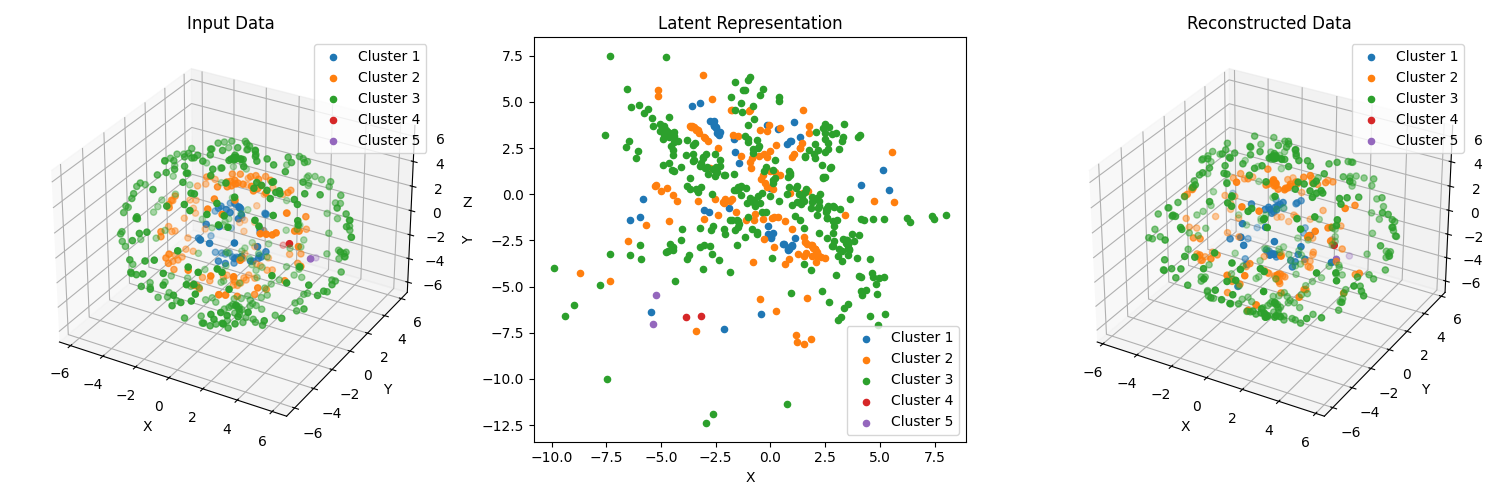
\includegraphics[width=\linewidth]{images/RQ2/mse/3DSphere_-1_0.0902.png}
    \caption{n=492 with 0.0902 MSE.}
    \label{fig:RQ2/mse/3DSphere}
  \end{subfigure}
  \hfill
  % subfigure 2
  \begin{subfigure}[b]{1.0\textwidth}
    \centering
    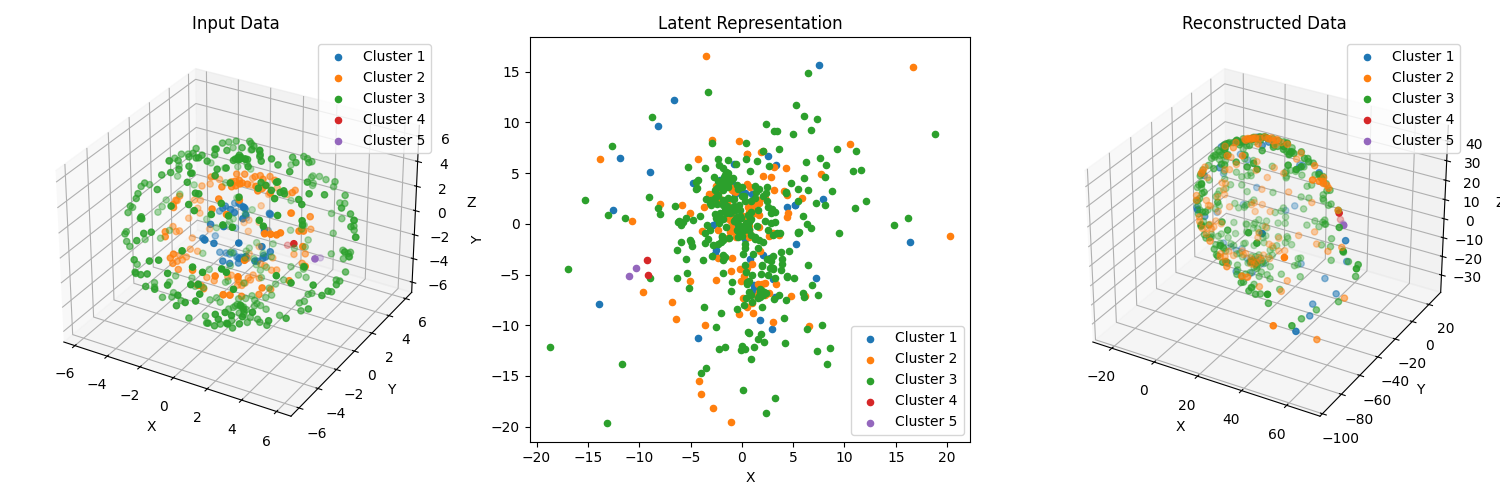
\includegraphics[width=\linewidth]{images/RQ2/csi/3DSphere_2_0.0009.png}
    \caption{n=492 with 0.0009 CosSim.}
    \label{fig:RQ2/csi/3DSphere}
  \end{subfigure}
  \hfill
  % subfigure 3
  \begin{subfigure}[b]{1.0\textwidth}
    \centering
    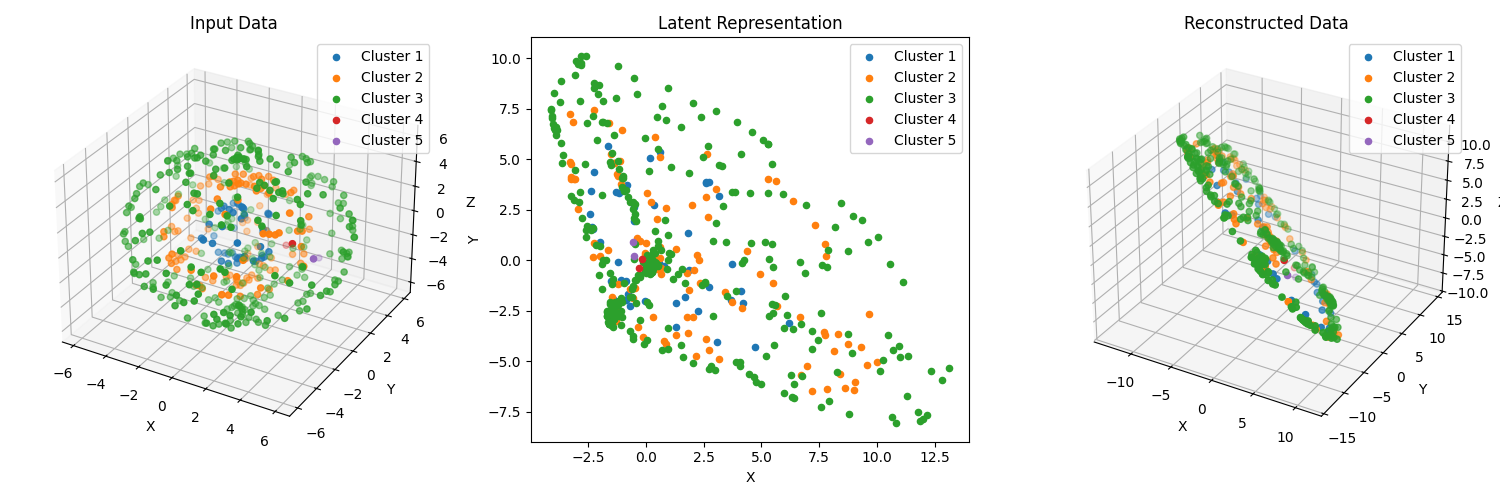
\includegraphics[width=\linewidth]{images/RQ2/kld/3DSphere_-1_0.0008.png}
    \caption{n=492 with 0.0008 KLD.}
    \label{fig:RQ2/kld/3DSphere}
  \end{subfigure}
  \hfill
  % subfigure 4
  \begin{subfigure}[b]{1.0\textwidth}
    \centering
    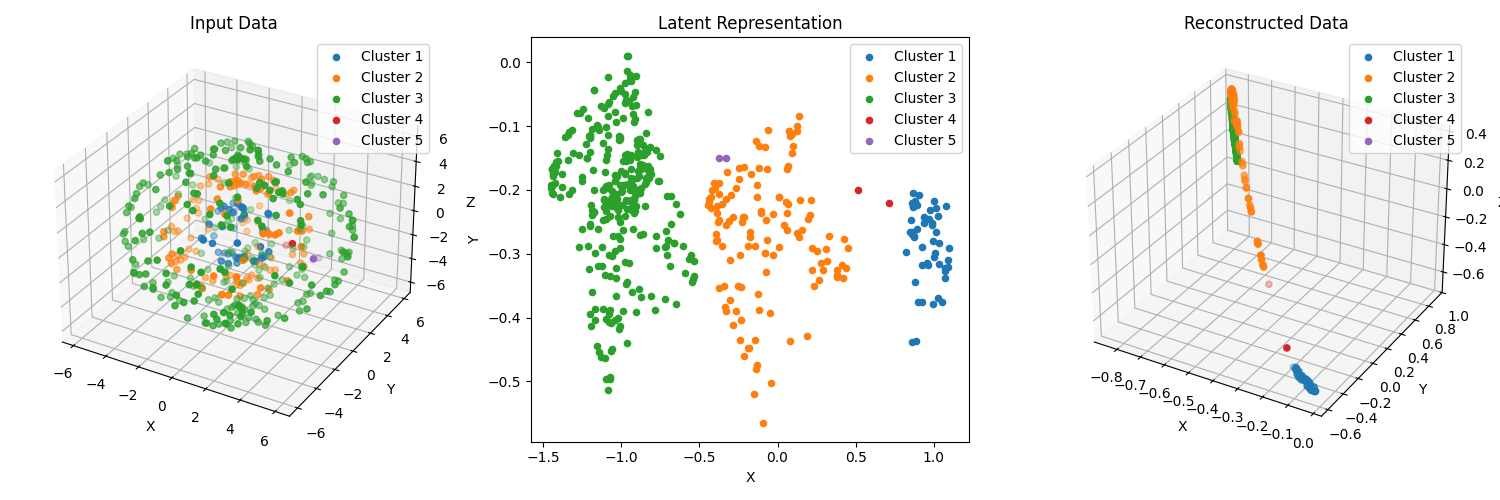
\includegraphics[width=\linewidth]{images/RQ2/tru/3DSphere_256n_32k_3.5759.png}
    \caption{n=256, k=32 with 3.5759 softTW.}
    \label{fig:RQ2/tru/3DSphere}
  \end{subfigure}

  \caption{Comparison of 3DSphere dataset (492 instances) experiments with different unsupervised loss functions.}
  \label{fig:RQ2/3DSphere}
\end{figure}

The \textbf{3DSphere} (Dataset \ref{fig:3DSphere}, Experiment \ref{fig:RQ2/3DSphere}) dataset presents a particularly challenging case because of its encapsulated structure: clusters are nested within one another like a set of matryoshka dolls. This configuration complicates the task of both reconstruction and embedding, since the model must compress a hierarchy of concentric relationships into a two-dimensional latent space. The expectation would be that an effective loss function should not only preserve the separation between the nested clusters but also represent the IBIs as bridges between them, all while capturing the global spherical geometry.

MSE, which had performed consistently well across simpler datasets, struggles with this more complex case. In the latent space, the embedding shows little evidence of circular organization. Instead, points appear scattered without a discernible spherical structure, and the IBIs are placed outside of this disorganized cloud rather than in positions that would connect the clusters meaningfully. Interestingly, the reconstruction does not reflects difficulties, to capture the nested structure in a coherent way. Cosine similarity produces very similar outcomes in the latent embedding, with scattered points and no clear structural continuity. Its reconstruction is waek, further underscoring its limitations in this highly complex, encapsulated geometry.

KLD provides a surprising contrast. In its low-dimensional embedding, a circular structure can still be observed, suggesting that this loss is better able to preserve aspects of the spherical arrangement than MSE or cosine similarity. Although the representation is far from perfect, the preservation of circularity marks a notable improvement over the more disordered embeddings of the other losses. The IBIs, however, are not positioned in a way that strongly reinforces their transitional role, limiting the interpretive value of this otherwise promising result.

The soft trustworthiness loss performs in a distinct manner. Here, the clusters are separated completely, with clear distinctions between them visible in the embedding. The IBIs occupy positions that serve as bridges between these separated groups, reflecting their intended transitional function more successfully than under the other losses. At the same time, however, the global circular structure of the spheres is lost, meaning that while the dataset is decomposed into distinct components, the nested, matryoshka-like character of the data is not preserved. This outcome highlights both the strengths and limitations of soft trustworthiness: it can enforce local separation and transitional bridging effectively, but it does so at the cost of global geometric fidelity.

Taken together, the results for the 3DSphere dataset emphasize the difficulty of encapsulated structures for autoencoder models and their loss functions. MSE and cosine similarity, typically reliable, fail to capture the circular organization and produce scattered embeddings with poorly placed IBIs. KLD surprisingly retains a degree of circular structure in its embedding, offering a more faithful representation than expected, though its treatment of IBIs remains limited. Soft trustworthiness, meanwhile, excels in separating clusters and embedding IBIs as bridges, but it fails to preserve the dataset’s global spherical organization. This dataset therefore reveals a divergence in the strengths of the different loss functions: while MSE is normally dominant, here KLD and soft trustworthiness each demonstrate specific advantages, suggesting that for highly encapsulated geometries, hybrid or alternative approaches may be required to balance global structure with transitional fidelity.
\newline

Across all experiments, clear differences emerged in the behavior and effectiveness of the four investigated loss functions, each demonstrating particular strengths and weaknesses depending on the dataset complexity and dimensionality.

The \textbf{mean squared error (MSE)} loss consistently proved to be the most reliable and robust objective. When trained with full-batch optimization, it not only delivered the fastest convergence but also produced the most faithful embeddings and reconstructions across nearly all datasets. Its reconstructions consistently matched the global geometry of the original data, and in the three-dimensional autoencoder setting, where the model had greater representational capacity, it demonstrated particularly strong performance. Importantly, MSE showed resilience even on highly complex datasets such as the 3DTorus, where it effectively separated the interwoven manifolds, and the 3DSwissRoll, where it reproduced the spiral structure faithfully. Although some limitations were observed, for instance in reconstructing the full width of clusters in the Moons datasets or in unrolling the Swiss rolls, MSE nevertheless stood out as the most consistent loss, making it the benchmark against which the others could be compared.

\textbf{Cosine similarity} exhibited behavior that was often comparable to MSE, though generally weaker, particularly in highly non-linear cases. On datasets such as 2DMoons, 2DSwissRoll, 3DSwissRoll, and 3DTorus, cosine similarity struggled to capture the same degree of structural fidelity. Its reconstructions tended to remain in the original input dimensionality, but the manifold complexity was consistently lower than that achieved by MSE. While the embeddings still separated clusters reasonably well in simpler datasets and positioned IBIs in a broadly acceptable manner, distortions appeared more frequently. For instance, in the Moons datasets, cosine similarity misplaced IBIs within clusters rather than between them, and in the Torus dataset it failed to separate the two interwoven rings. As such, cosine similarity can be seen as a lighter-weight alternative to MSE that performs adequately in less demanding settings but loses reliability as structural complexity increases.

The \textbf{Kullback–Leibler divergence (KLD)} produced the weakest results overall. Across all datasets, from the simplest Gaussian blobs to the most intricate manifold structures, reconstructions under KLD consistently collapsed onto a space of one dimension lower than the input. This systematic reduction in dimensionality points to a consistent loss of information during training. In the latent space, clusters frequently merged together, obscuring both cluster identity and the transitional role of IBIs. These failures were not limited to complex cases such as the Swiss rolls or the Torus but also occurred in simple settings like 2DBlobsS and 2DBlobsM, where one would otherwise expect straightforward separability. Even in three-dimensional extensions of these datasets, the same pattern persisted, with cluster overlap and misplaced IBIs. This consistent underperformance highlights KLD’s unsuitability for tasks requiring faithful preservation of cluster structure and transitional relationships, particularly when compared with the stability of MSE.

The \textbf{soft trustworthiness (softTW)} objective displayed a much more inconsistent and parameter-sensitive behavior. Unlike the other losses, it introduced an additional parameter, the neighborhood size k, which, together with the batch size, heavily influenced results. This sensitivity meant that performance could vary widely between runs, and the absolute loss values could not be meaningfully compared across experiments. Reconstructions under softTW almost invariably collapsed onto one-dimensional manifolds, regardless of the input dimensionality. This reflects the local nature of the objective: it emphasizes preservation of neighborhood relations at the expense of global structure. As a result, overall cluster shapes were almost always lost in the low-dimensional embeddings, even when local continuity was preserved. Nevertheless, in specific cases softTW demonstrated remarkable potential. It was the only objective that managed to unroll the 3DSwissRoll, even if the reconstruction was poor. It also separated the interwoven rings of the 3DTorus to some extent and performed particularly well on the 3DSphere dataset, where it successfully separated the encapsulated spheres and positioned IBIs as bridges. These isolated successes suggest that while softTW is unreliable in isolation, it may hold promise as part of a hybrid loss function. In particular, combining MSE to capture global structure with softTW to refine local relationships could yield models that balance fidelity with neighborhood preservation, a direction that merits future exploration.

Taken together, these results establish a clear hierarchy of performance. MSE emerges as the most stable and effective loss function, capable of handling a wide range of dataset complexities with reliable accuracy. Cosine similarity provides a weaker but still serviceable alternative, particularly in simpler scenarios. KLD consistently underperforms, collapsing dimensionality and merging clusters in ways that obscure both global and transitional structures. Soft trustworthiness, while inconsistent and highly sensitive to parameters, demonstrates unique strengths in certain situations, hinting at its potential when integrated into a combined objective. This comparative analysis thus not only confirms the primacy of MSE but also points toward future directions in which complementary losses might be combined to capture both global and local structures in a more balanced fashion.